\section*{Introduction}
\addcontentsline{toc}{section}{Introduction}

This sprint report covers \textbf{Domain 3: Production Execution \& Traceability}.
Building upon the authentication and machine monitoring infrastructure established
in the previous sprints, this sprint delivers the core production execution
features; declaring production output, pausing and resuming operations, finishing, Interrupting 
or cancelling orders, tracking production declarations over time, monitoring Bill of
Materials consumption, component barcode scanning, scrap declaration, supervisor
proxy declaration, and label printing. The result is a fully operational shop-floor
execution loop from order assignment through to order closure, material traceability,
and printed part identification.

% ---------------------------------------------------------------------------
% 1. SPRINT BACKLOG
% ---------------------------------------------------------------------------
\section{Sprint Backlog}

This sprint covers \textbf{Domain 3:} \textbf{\domainterm{Production Execution \& Traceability}}.

% ----------------------------------------------------------
% US-3.1
% ----------------------------------------------------------
\begin{longtable}{@{} P{0.09\linewidth} P{0.38\linewidth} P{0.49\linewidth} @{}}
	\caption{US-3.1 --- Declare Production}
	\label{tab:s3-US-3.1} \\
	\toprule
	\textbf{ID} & \textbf{User Story} & \textbf{Tasks} \\
	\midrule
	\endfirsthead
	\toprule
	\textbf{ID} & \textbf{User Story} & \textbf{Tasks} \\
	\midrule
	\endhead
	\multicolumn{3}{r}{\small Continued on next page} \\
	\endfoot
	\bottomrule
	\endlastfoot
	
	\textbf{US-3.1}
	& As an \userrole{Operator} or \userrole{Supervisor}, I need to declare the
	produced quantity in a cycle so that the system records my
	production progress.
	& \noindent\textit{Business Central (AL):}
	\begin{itemize}[noitemsep, topsep=0pt, partopsep=0pt, leftmargin=*]
		\item Create table \techname{MES Operation Progression}.
		\item Create the functions:
		\begin{itemize}[noitemsep, topsep=0pt, partopsep=0pt, leftmargin=*]
			\item \texttt{TryDeclareProduction()} in codeunit \techname{MESMachineValidation}.
			\item \texttt{InsertNewProgressionCycle()} in codeunit \techname{MESMachineInsert}.
			\item \texttt{declareProduction()} in codeunit \techname{MESMachineWrite}.
		\end{itemize} 
		\item Expose \texttt{declareProduction()} through the codeunit \techname{MES Web Service}.
		\item Create page \techname{MES Operation Progression} list page.
	\end{itemize}
	\\ & &
	\noindent\textit{Flutter:}
	\begin{itemize}[noitemsep, topsep=0pt, partopsep=0pt, leftmargin=*]
		\item Updated \techname{ErpMachineOrdersService} to consume the \texttt{declareProduction} API and \techname{MachineordersProvider} to manage it.
	\end{itemize}
	\\ & &
	\noindent\textit{Flutter(continuation):}
	\begin{itemize}[noitemsep, topsep=0pt, partopsep=0pt, leftmargin=*]
		\item Create widget \techname{DeclareProductionDialog}.
		\item Add the \texttt{Declare Production} action in \techname{ActionButtonsContainer}.
	\end{itemize}\\
	\midrule
	\textbf{US-3.2}
	& As an \userrole{Operator} or \userrole{Supervisor}, I need to pause and
	resume an active operation so that production interruptions are tracked
	accurately.
	& \noindent\textit{Business Central (AL):}
	\begin{itemize}[noitemsep, topsep=0pt, partopsep=0pt, leftmargin=*]
		\item Create the functions:
		\begin{itemize}[noitemsep, topsep=0pt, partopsep=0pt, leftmargin=*] 
			\item \texttt{TryPauseOperation()} and \texttt{TryResumeOperation()} in codeunit \techname{MESMachineValidation}.
			\item \texttt{ExecuteOperationTransition()}, \texttt{pauseOperation()}, and \texttt{resumeOperation()} in codeunit \techname{MESMachineWrite}. 
		\end{itemize}
		\item Expose \texttt{pauseOperation()} and \texttt{resumeOperation()} throught codeunit \techname{MES Web Service}.
	\end{itemize}
	\\ & &
	\noindent\textit{Flutter:}
	\begin{itemize}[noitemsep, topsep=0pt, partopsep=0pt, leftmargin=*]
		\item Implement \techname{ErpMachineOrdersService} to consume the new endpoints 
		\item Implement \techname{MachineordersProvider} to manage its state.
		\item Create widget \techname{OperationActionButtons}.
		\item Implement pause/resume operation toggle handling in \techname{OrdersProgressionPage}.
	\end{itemize} \\
	\midrule
	\textbf{US-3.3}
	& As a \userrole{Supervisor}, I need to finish, interrupt or cancel a production
	operation so that the machine is released and the order is closed in the
	system.
	& \noindent\textit{Business Central (AL):}
	\begin{itemize}[noitemsep, topsep=0pt, partopsep=0pt, leftmargin=*]
		\item Create the functions:
		\begin{itemize}[noitemsep, topsep=0pt, partopsep=0pt, leftmargin=*]
			\item \texttt{TryCloseOperation()} in codeunit \techname{MESMachineValidation}.
			\item \texttt{InsertOperationStatus()}, \texttt{SetErpOrderToFinish()}, \texttt{InsertStartMESMachineStatus()}  and \texttt{InsertIdleMachineStatus()} in codeunit \techname{MESMachineInsert}.
			\item \texttt{finishOperation()} and \texttt{cancelOperation()} in codeunit \techname{MESMachineWrite}.
			\item \texttt{ExecuteCancelUnstartedOperation()} in codeunit \techname{MESMachineWrite}.
		\end{itemize}
		\item Expose \texttt{finishOperation()} and \texttt{cancelOperation()} in codeunit \techname{MES Web Service}.
	\end{itemize}
\\ & &
	\noindent\textit{Flutter:}
	\begin{itemize}[noitemsep, topsep=0pt, partopsep=0pt, leftmargin=*]
		\item Update \techname{ErpMachineOrdersService} to consume the new endpoints.
		\item Update \techname{MachineOrdersProvider} to manage its state.
		\item Update \techname{ActionButtonsContainer} to handle Finish/Interrupt operation flow.
	\end{itemize} \\
	\midrule
	\textbf{US-3.4}
	& As an \userrole{Operator} or \userrole{Supervisor}, I need a dedicated
	detail page for an operation so that I can see all real-time information
	in one place.
	& \noindent\textit{Business Central (AL):}
	\begin{itemize}[noitemsep, topsep=0pt, partopsep=0pt, leftmargin=*]
		\item Create table \techname{MES Operation Execution}.
		\item Create function \texttt{InsertMESOperationExecution()} in codeunit \techname{MESMachineInsert}.
		\item Create function \texttt{fetchOperationLiveData()} in codeunit \techname{MESMachineFetch}.
		\item Expose \texttt{fetchOperationLiveData()} through codeunit \techname{MES Web Service}.
		\item Create page \techname{MES Operation Execution}.
	\end{itemize}
\\ & &
	\noindent\textit{Flutter:}
	\begin{itemize}[noitemsep, topsep=0pt, partopsep=0pt, leftmargin=*]
		\item Create model \techname{OperationStatusAndProgressModel}.
		\item Update \techname{ErpMachineOrdersService} to consume the new endpoints.
		\item Update \techname{MachineOrdersProvider} to manage its state.
		\item Create page \techname{OperationDetailPage}.
		\item Create widget \techname{OperationAppBar}.
		\item Create widget \techname{CurrentOrderInfoContainer}.
	\end{itemize}\\
	\midrule
	
	\textbf{US-3.5}
	& As an \userrole{Operator} or \userrole{Supervisor}, I need to see all
	production cycles declared for an operation so that I can review each
	declaration's quantity, operator, and timestamp.
	& \noindent\textit{Business Central (AL):}
	\begin{itemize}[noitemsep, topsep=0pt, partopsep=0pt, leftmargin=*]
		\item Create function \texttt{fetchProductionCycles()} in codeunit \techname{MESMachineFetch}.
		\item Expose \texttt{fetchProductionCycles()} throught codeunit \techname{MES Web Service}.
	\end{itemize}
\\ & &
	\noindent\textit{Flutter:}
	\begin{itemize}[noitemsep, topsep=0pt, partopsep=0pt, leftmargin=*]
		\item Create model \techname{ProductionCycleModel}.
		\item Update \techname{ErpMachineOrdersService} to consume the new endpoints.
		\item Update \techname{MachineOrdersProvider} to manage its state.
		\item Create widget \techname{ProductionCycle}.
	\end{itemize} \\
\midrule
	
	\textbf{US-3.6}
	& As an \userrole{Operator} or \userrole{Supervisor}, I need to see a visual
	chart of production declarations over time so that I can identify trends
	and performance patterns.
	& \noindent\textit{Flutter:}
	\begin{itemize}[noitemsep, topsep=0pt, partopsep=0pt, leftmargin=*]
		\item Create widget \techname{ProductionChart}.
		\item create a function to ensure that the chart is always centered
		\item implemented a scrollable view into the chart
	\end{itemize}\\
	\midrule
	\textbf{US-3.7}
	& As an \userrole{Operator} or \userrole{Supervisor}, I need to see the
	Bill of Materials for a production operation so that I know which
	components are required, how much has already been consumed, and the amount 
	available in the inventory.
	& \noindent\textit{Business Central (AL):}
	\begin{itemize}[noitemsep, topsep=0pt, partopsep=0pt, leftmargin=*]
		\item Create function \texttt{fetchBom()} in codeunit \techname{MESMachineFetch}.
		\item Expose \texttt{fetchBom()} through codeunit \techname{MES Web Service}.
		
	\end{itemize}
\\ & &
	\noindent\textit{Flutter:}
	\begin{itemize}[noitemsep, topsep=0pt, partopsep=0pt, leftmargin=*]
		\item Create \techname{MesComponentConsumptionService} to consume the \texttt{fetchBom()} API.
		\item Create \techname{MesComponentConsumptionProvider} to manage BOM stream and refresh state.
		\item Create widget \techname{RequiredComponent}.
		\item Implement BOM streaming and refresh flow in \techname{MesComponentConsumptionService} and \techname{MesComponentConsumptionProvider}.
		\item Implement component status display and operation-based filtering in \techname{RequiredComponent} widget.
	\end{itemize}\\
	\midrule
	\textbf{US-3.8}
	& As an \userrole{Operator} or \userrole{Supervisor}, I need to report
	scrapped units with a reason code so that waste is accurately tracked.
	& \noindent\textit{Business Central (AL):}
	\begin{itemize}[noitemsep, topsep=0pt, partopsep=0pt, leftmargin=*]
		\item Create table \techname{MES Operation Scrap}.
		\item Create function \texttt{declareScrap()} in codeunit \techname{MES Machine Write}.
		\item Expose \texttt{declareScrap()} through codeunit \techname{MES Web Service}.
		\item Create \techname{MES Scrap Code API} to fetch scrap codes from the standard \techname{Business Central} \modulename{Scrap Code}.
	\end{itemize}
\\ & &
	\noindent\textit{Flutter:}
	\begin{itemize}[noitemsep, topsep=0pt, partopsep=0pt, leftmargin=*]
		\item Create model \techname{MesScrapCode}.
		\item Create \techname{MesScrapService} to consume the scrap code fetch and \texttt{declareScrap()} APIs.
		\item Create \techname{MesScrapProvider} to manage scrap code and scrap declaration state.
		\item Create dialog \techname{DeclareScrapDialog}.
	\end{itemize}\\
	\midrule
	\textbf{US-3.9}
	& As a \userrole{Supervisor}, I need to declare production on behalf of an
	operator so that output is attributed to the correct person.
	& \noindent\textit{Business Central (AL):}
	\begin{itemize}[noitemsep, topsep=0pt, partopsep=0pt, leftmargin=*]
		\item Add field \texttt{Declared By} to the tables \techname{MES Operation Progression} and \techname{MES Operation Scan}.
	\end{itemize}
\\ & &
	\noindent\textit{Flutter:}
	\begin{itemize}[noitemsep, topsep=0pt, partopsep=0pt, leftmargin=*]
		\item Create widget \techname{OperatorSelector}.
		\item Update \techname{DeclareProductionDialog} to support supervisor declaration on behalf of an operator.
		\item Connect \techname{OperatorSelector} to \techname{MesUserProvider} and pass \texttt{onBehalfOfUserId} to \techname{MachineOrdersProvider.declareProduction()}.
	\end{itemize} \\
	\midrule
	\textbf{US-3.10}
	& As an \userrole{Operator} or \userrole{Supervisor}, I need to scan
	components into an operation so that consumption is recorded against the BOM.
	& \noindent\textit{Business Central (AL):}
	\begin{itemize}[noitemsep, topsep=0pt, partopsep=0pt, leftmargin=*]
		\item Create table \techname{MES Component Scan}.
		\item Create the function \texttt{insertScans()} in codeunit \techname{MES Machine Write}.
		\item Create the functions  \texttt{resolveBarcode()} in codeunit \techname{MES Machine Fetch}.
		\item Expose the three function through codeunit \techname{MES Web Service}.
		\item Create page \techname{MES Component Consumption}.
	\end{itemize}
\\ & &
	\noindent\textit{Flutter:}
	\begin{itemize}[noitemsep, topsep=0pt, partopsep=0pt, leftmargin=*]
		\item Create model \techname{ItemBarcodeModel}.
		\item Create \techname{MesBarcodeService} to consume the endpoints \texttt{insertScans()}, and \texttt{resolveBarcode()}.
		\item Create \techname{MesBarcodeProvider} to manage barcode state and API calls.
		\item Create widget \techname{ScannerWidget}.
		\item Update widget \techname{RequiredComponent} to integrate item scanning, search, filtering, and BOM refresh after scan submission.
		\item Implement on\-device camera scanning via \techname{mobile\_scanner} in \techname{ScannerWidget}
	\end{itemize}\\
	\midrule
	\textbf{US-3.11}
	& As an \userrole{Operator} or \userrole{Supervisor}, I need to print a label
	for the finished production operations (100\% progress) so that produced parts are correctly identified.
	& \noindent\textit{Flutter:}
	\begin{itemize}[noitemsep, topsep=0pt, partopsep=0pt, leftmargin=*]
		\item Create page \techname{PrintLabelPage}.
		\item Update \techname{ActionButtonsContainer} to integrate the \uilabel{Print Label} action.
		\item Implement label generation, preview, print flow, and orientation toggle in \techname{PrintLabelPage}.
	\end{itemize} \\
	\midrule
	\textbf{US-3.12}
	& As an \userrole{Operator} or \userrole{Supervisor}, I need a label printed
	for each declared unit so that individual pieces carry traceable information.
	& \noindent\textit{Flutter:}
	\begin{itemize}[noitemsep, topsep=0pt, partopsep=0pt, leftmargin=*]
		\item Create page \techname{DeclarationLabelPage}.
		\item Implement declaration label generation, preview, orientation toggle, and per-unit PDF export in \techname{DeclarationLabelPage}.
	\end{itemize} \\
\end{longtable}


\section{Design}

\subsection{Use Case Diagram}

\noindent
\vspace{0pt}
This sprint adds production execution actors and interactions centred on the \userrole{Operator}
and \userrole{Supervisor} roles. The primary use cases are: Declare Production, Pause Operation,
Resume Operation, Finish Operation, Interrupt Operation, Cancel Operation, View BOM Components, 
View Operation Detail, View declaration History.

The \userrole{Supervisor} role is a superset of \userrole{Operator}: both roles can declare production,
pause, resume, and view detail; only the Supervisor may close (Finish, Interrupt or Cancel) a production order
in the intended business flow, although the current implementation enforces this at the UI layer 
through the \texttt{canCloseProductionOrder} flag rather than at the API level. The resulting use 
case diagram is shown in Figures~\ref{fig:s3-uc-part1} and~\ref{fig:s3-uc-part2}.

\begin{figure}[H]
  \centering
  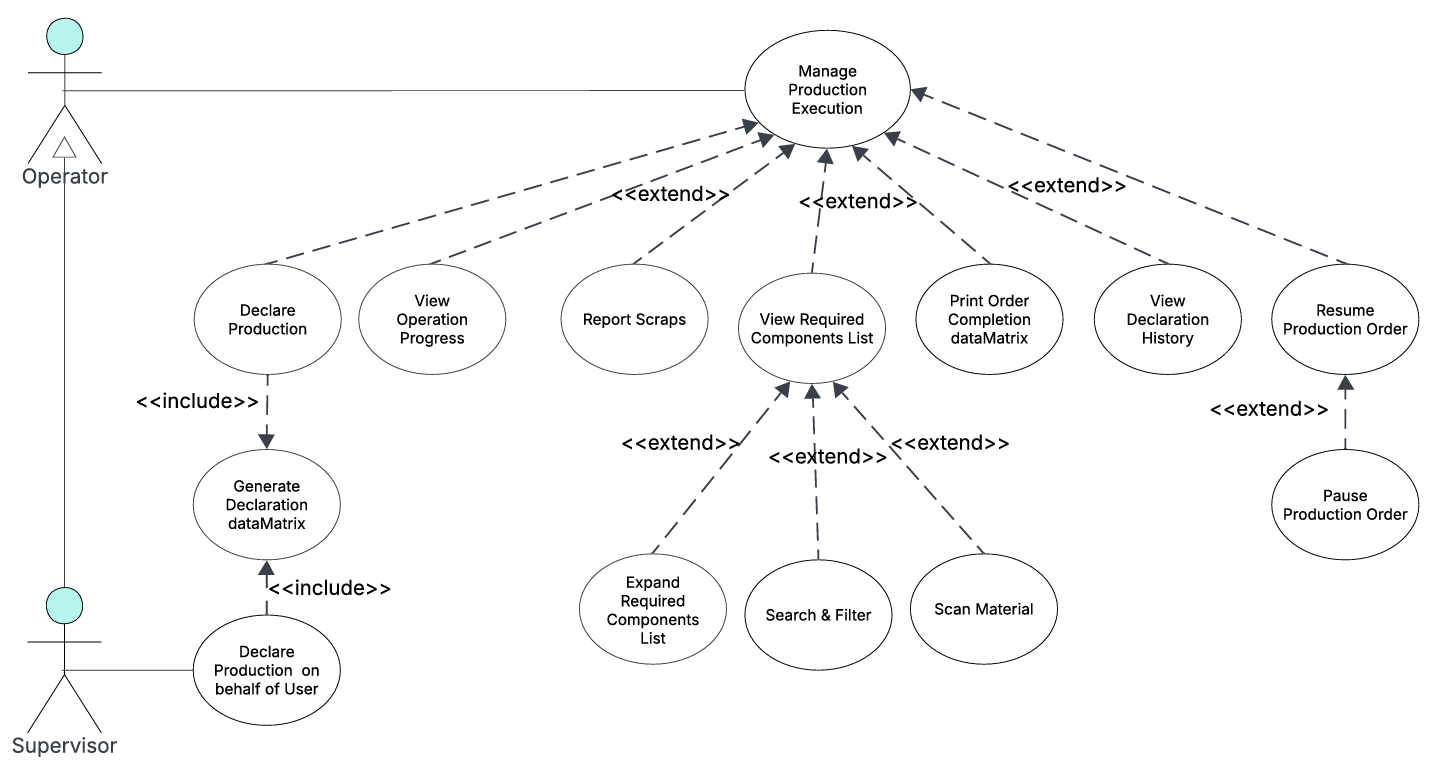
\includegraphics[width=\linewidth,keepaspectratio]{./media/MES_Sprint-3-Repport/diagrams/useCase/sprint3-1.png}
  \caption{UML Use Case Diagram --- Sprint 3 (manage production)}
  \label{fig:s3-uc-part1}
\end{figure}

\begin{figure}[H]
  \centering
  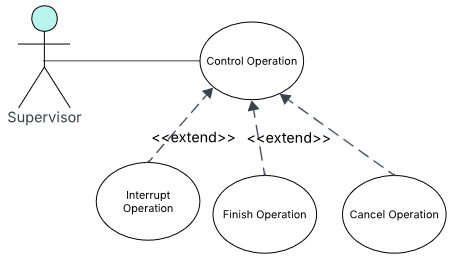
\includegraphics[height=0.35\textheight,keepaspectratio]{./media/MES_Sprint-3-Repport/diagrams/useCase/sprint3-2.png}
  \caption{UML Use Case Diagram --- Sprint 3 (control operations)}
  \label{fig:s3-uc-part2}
\end{figure}

\subsection{Textual Use Case Description}

\Needspace{10\baselineskip}
\begin{longtable}{@{} P{0.21\linewidth} P{0.75\linewidth} @{}}
	\caption{Textual Use Case Description --- Declare Production}
	\label{tab:s3-uc-declare-production} \\
	\toprule
	\endfirsthead
	\midrule
	\endhead
	
	\multicolumn{2}{r}{\small Continued on next page} \\
	\endfoot
	\bottomrule
	\endlastfoot
	
	\textbf{Use Case Name} & Declare Production \\
	\midrule
	\textbf{Primary Actor} & \userrole{Operator} / \userrole{Supervisor} \\
	\midrule
	\textbf{Preconditions} & 
	\begin{itemize}[noitemsep, topsep=0pt, partopsep=0pt, leftmargin=*]
	\item The user is authenticated and navigated to an Operation Detail page.
	\item The operation status is \domainterm{Running}.
	\item The produced quantity is below the order quantity.
	\end{itemize} \\
	\midrule
	\textbf{Postconditions} & 
	\begin{itemize}[noitemsep, topsep=0pt, partopsep=0pt, leftmargin=*]
	\item A new \techname{MES Operation Progression} record is inserted.
	\item The production chart and cycle table update via the refresh stream or trigger.
	\item The progress percentage and produced quantity in the info container update.
	\end{itemize} \\
	\midrule
	\textbf{Main Scenario} & 
	\begin{enumerate}[noitemsep, topsep=0pt, partopsep=0pt, leftmargin=*]
	\item The user taps \uilabel{Declare Production} in the Quick Actions panel.
	\item The \techname{DeclareProductionDialog} opens showing the remaining quantity.
	\item The user (if Supervisor) optionally selects an operator from the dropdown to declare on behalf of.
	\item The user enters a positive integer not exceeding the remaining quantity.
	\item The user taps \uilabel{Submit}.
	\item The ERP validates the quantity and inserts the progression record.
	\item The user is redirected to the declaration lable print page
	\item The refresh stream triggers a live data update.
	\end{enumerate} \\
	\midrule
	\textbf{Alternative Flow} & 
	\begin{itemize}[noitemsep, topsep=0pt, partopsep=0pt, leftmargin=*]
	\item \textit{Step 3, invalid quantity}: client-side validation shows an inline error; submission is blocked.
	\item \textit{Step 6, ERP error}: the server error message is displayed in the dialog; the record is not inserted.
	\end{itemize} \\
\end{longtable}


\bigskip

\Needspace{10\baselineskip}
\begin{longtable}{@{} P{0.21\linewidth} P{0.75\linewidth} @{}}
	\caption{Textual Use Case Description --- Finish / Cancel / Interrupt Operation}
	\label{tab:s3-uc-close-operation} \\
	\toprule
	\endfirsthead
	\midrule
	\endhead
	\multicolumn{2}{r}{\small Continued on next page} \\
	\endfoot
	\bottomrule
	\endlastfoot
	
	\textbf{Use Case Name} & Finish / Cancel / Interrupt Operation \\
	\midrule
	\textbf{Primary Actor} & \userrole{Supervisor} \\
	\midrule
	\textbf{Preconditions} & 
	\begin{itemize}[noitemsep, topsep=0pt, partopsep=0pt, leftmargin=*]
	\item The user is authenticated with an active session as a \userrole{Supervisor}.
	\item The operation is in \domainterm{Running}, \domainterm{Paused}, or \domainterm{Released and unstarted} state.
	\end{itemize} \\
	\midrule
	\textbf{Postconditions} & 
	\begin{itemize}[noitemsep, topsep=0pt, partopsep=0pt, leftmargin=*]
	\item A \domainterm{Finished}, \domainterm{Interrupted}, or \domainterm{Cancelled} status record is inserted.
	\item The execution end time is stamped.
	\item An Idle machine status record is inserted if the operation was started.
	\end{itemize} \\
	\midrule
	\textbf{Main Scenario} & 
	\begin{enumerate}[noitemsep, topsep=0pt, partopsep=0pt, leftmargin=*]
	\item The user clickes in the (Interrupt, Finish, Cancel) button based on the operation state.
	\item A confirmation dialog is displayed; the user confirms.
	\item The system POSTs to \apiendpoint{/MESWebService\_finishOperation} or \apiendpoint{cancelOperation}.
	\item The ERP validates, inserts the status record, stamps the end time, and inserts an Idle machine status.
	\end{enumerate} \\
\end{longtable}


\Needspace{10\baselineskip}
\begin{longtable}{@{} P{0.21\linewidth} P{0.75\linewidth} @{}}
    \caption{Textual Use Case Description --- Scan Component Consumption}
    \label{tab:s3-uc-scan-component-consumption} \\
    \toprule
    \endfirsthead
    \midrule
    \endhead
    \multicolumn{2}{r}{\small Continued on next page} \\
    \endfoot
    \bottomrule
    \endlastfoot

    \textbf{Use Case Name} & Scan Component Consumption \\
    \midrule
    \textbf{Primary Actor} & \userrole{Operator} / \userrole{Supervisor} \\
    \midrule
    \textbf{Preconditions} &
    \begin{itemize}[noitemsep, topsep=0pt, partopsep=0pt, leftmargin=*]
        \item The user is authenticated and holds a valid session token.
        \item The operation has been started.
        \item The user is on the Operation Detail page with the \techname{ScannerWidget} open.
    \end{itemize} \\
    \midrule
    \textbf{Postconditions} &
    \begin{itemize}[noitemsep, topsep=0pt, partopsep=0pt, leftmargin=*]
        \item One \techname{MES Operation Scan} record is inserted per scanned item line.
        \item One \techname{Item Journal Line} (consumption) is posted to BC inventory per scanned item line.
        \item The \techname{Required Component} widget refreshes to reflect the updated consumed quantities.
    \end{itemize} \\
    \midrule
    \textbf{Main Scenario} &
    \begin{enumerate}[noitemsep, topsep=0pt, partopsep=0pt, leftmargin=*]
        \item The user taps \uilabel{Scan Item} and points the camera or scanner at a component barcode.
        \item Flutter POSTs to \apiendpoint{/api/resolveBarcode}; the middleware forwards the call to \techname{MESWebService\_resolveBarcode} in AL.
        \item AL resolves the item: if the barcode carries an \texttt{Item Number:} prefix, AL parses the item number directly and retrieves the item record from BC; otherwise AL resolves the identifier via the \techname{Item Identifier} table.
        \item AL fetches the unit-of-measure conversion factor via \texttt{Item Unit of Measure.Get} and returns \texttt{itemNo}, \texttt{itemDescription}, \texttt{unitOfMeasure}, and \texttt{quantityPerUnitOfMeasure} to Flutter.
        \item Flutter validates the response and adds the item to the local scanned-items list (or increments its quantity if already present); the item appears in the scan list.
        \item The user repeats steps 1--5 for each additional component, then taps \uilabel{Confirm Scans}.
        \item Flutter POSTs the full scan list to \apiendpoint{/api/insertScans}; the middleware forwards to \techname{MESWebService\_insertScans} in AL.
        \item AL for each scan inserts an \techname{MES Operation Scan} record and an \techname{Item Journal Line}.
        \item AL posts all journal lines to BC inventory in a single batch; BC confirms success.
        \item Flutter pops the \techname{ScannerWidget} and triggers a data refresh; the \techname{Required Component} widget displays the updated consumed quantities.
    \end{enumerate} \\
    \midrule
    \textbf{Alternative Flow} &
    \begin{itemize}[noitemsep, topsep=0pt, partopsep=0pt, leftmargin=*]
        \item \textit{Step 3, unresolvable barcode}: AL returns an error; Flutter displays an inline error message and does not add the item to the scan list.
        \item \textit{Step 5, client validation failure}: Flutter blocks the addition and shows an inline error (e.g.\ zero or negative quantity).
        \item \textit{Step 9, BC posting error}: AL returns the server error to Flutter; no consumption or journal records are committed, and the dialog remains open with the error displayed.
    \end{itemize} \\
\end{longtable}
\bigskip

\subsection{Sequence Diagrams}

The following sequence diagrams illustrate the communication flow between the
\techname{Flutter} frontend, the \techname{Business Central} OData layer, and
the \techname{AL} business logic for the production and operation-lifecycle
flows introduced in Sprint~3.

% Figure~\ref{fig:s3-seq-declare-production} depicts the production declaration
% flow. The operator submits a quantity; the \techname{Flutter} client validates
% the input locally, then forwards the request to the \techname{AL} layer,
% which re-validates the token (SD-02), checks that the declared amount is
% positive and does not exceed the remaining order quantity, and — on success —
% inserts a new immutable \domainterm{MES Operation Progression} record and
% records the relevant user interaction entries. When a \userrole{Supervisor}
% declares production on behalf of an operator, the \techname{AL} layer
% additionally verifies that the two users share at least one work centre before
% proceeding.

% \begin{figure}[H]
%   \centering
%   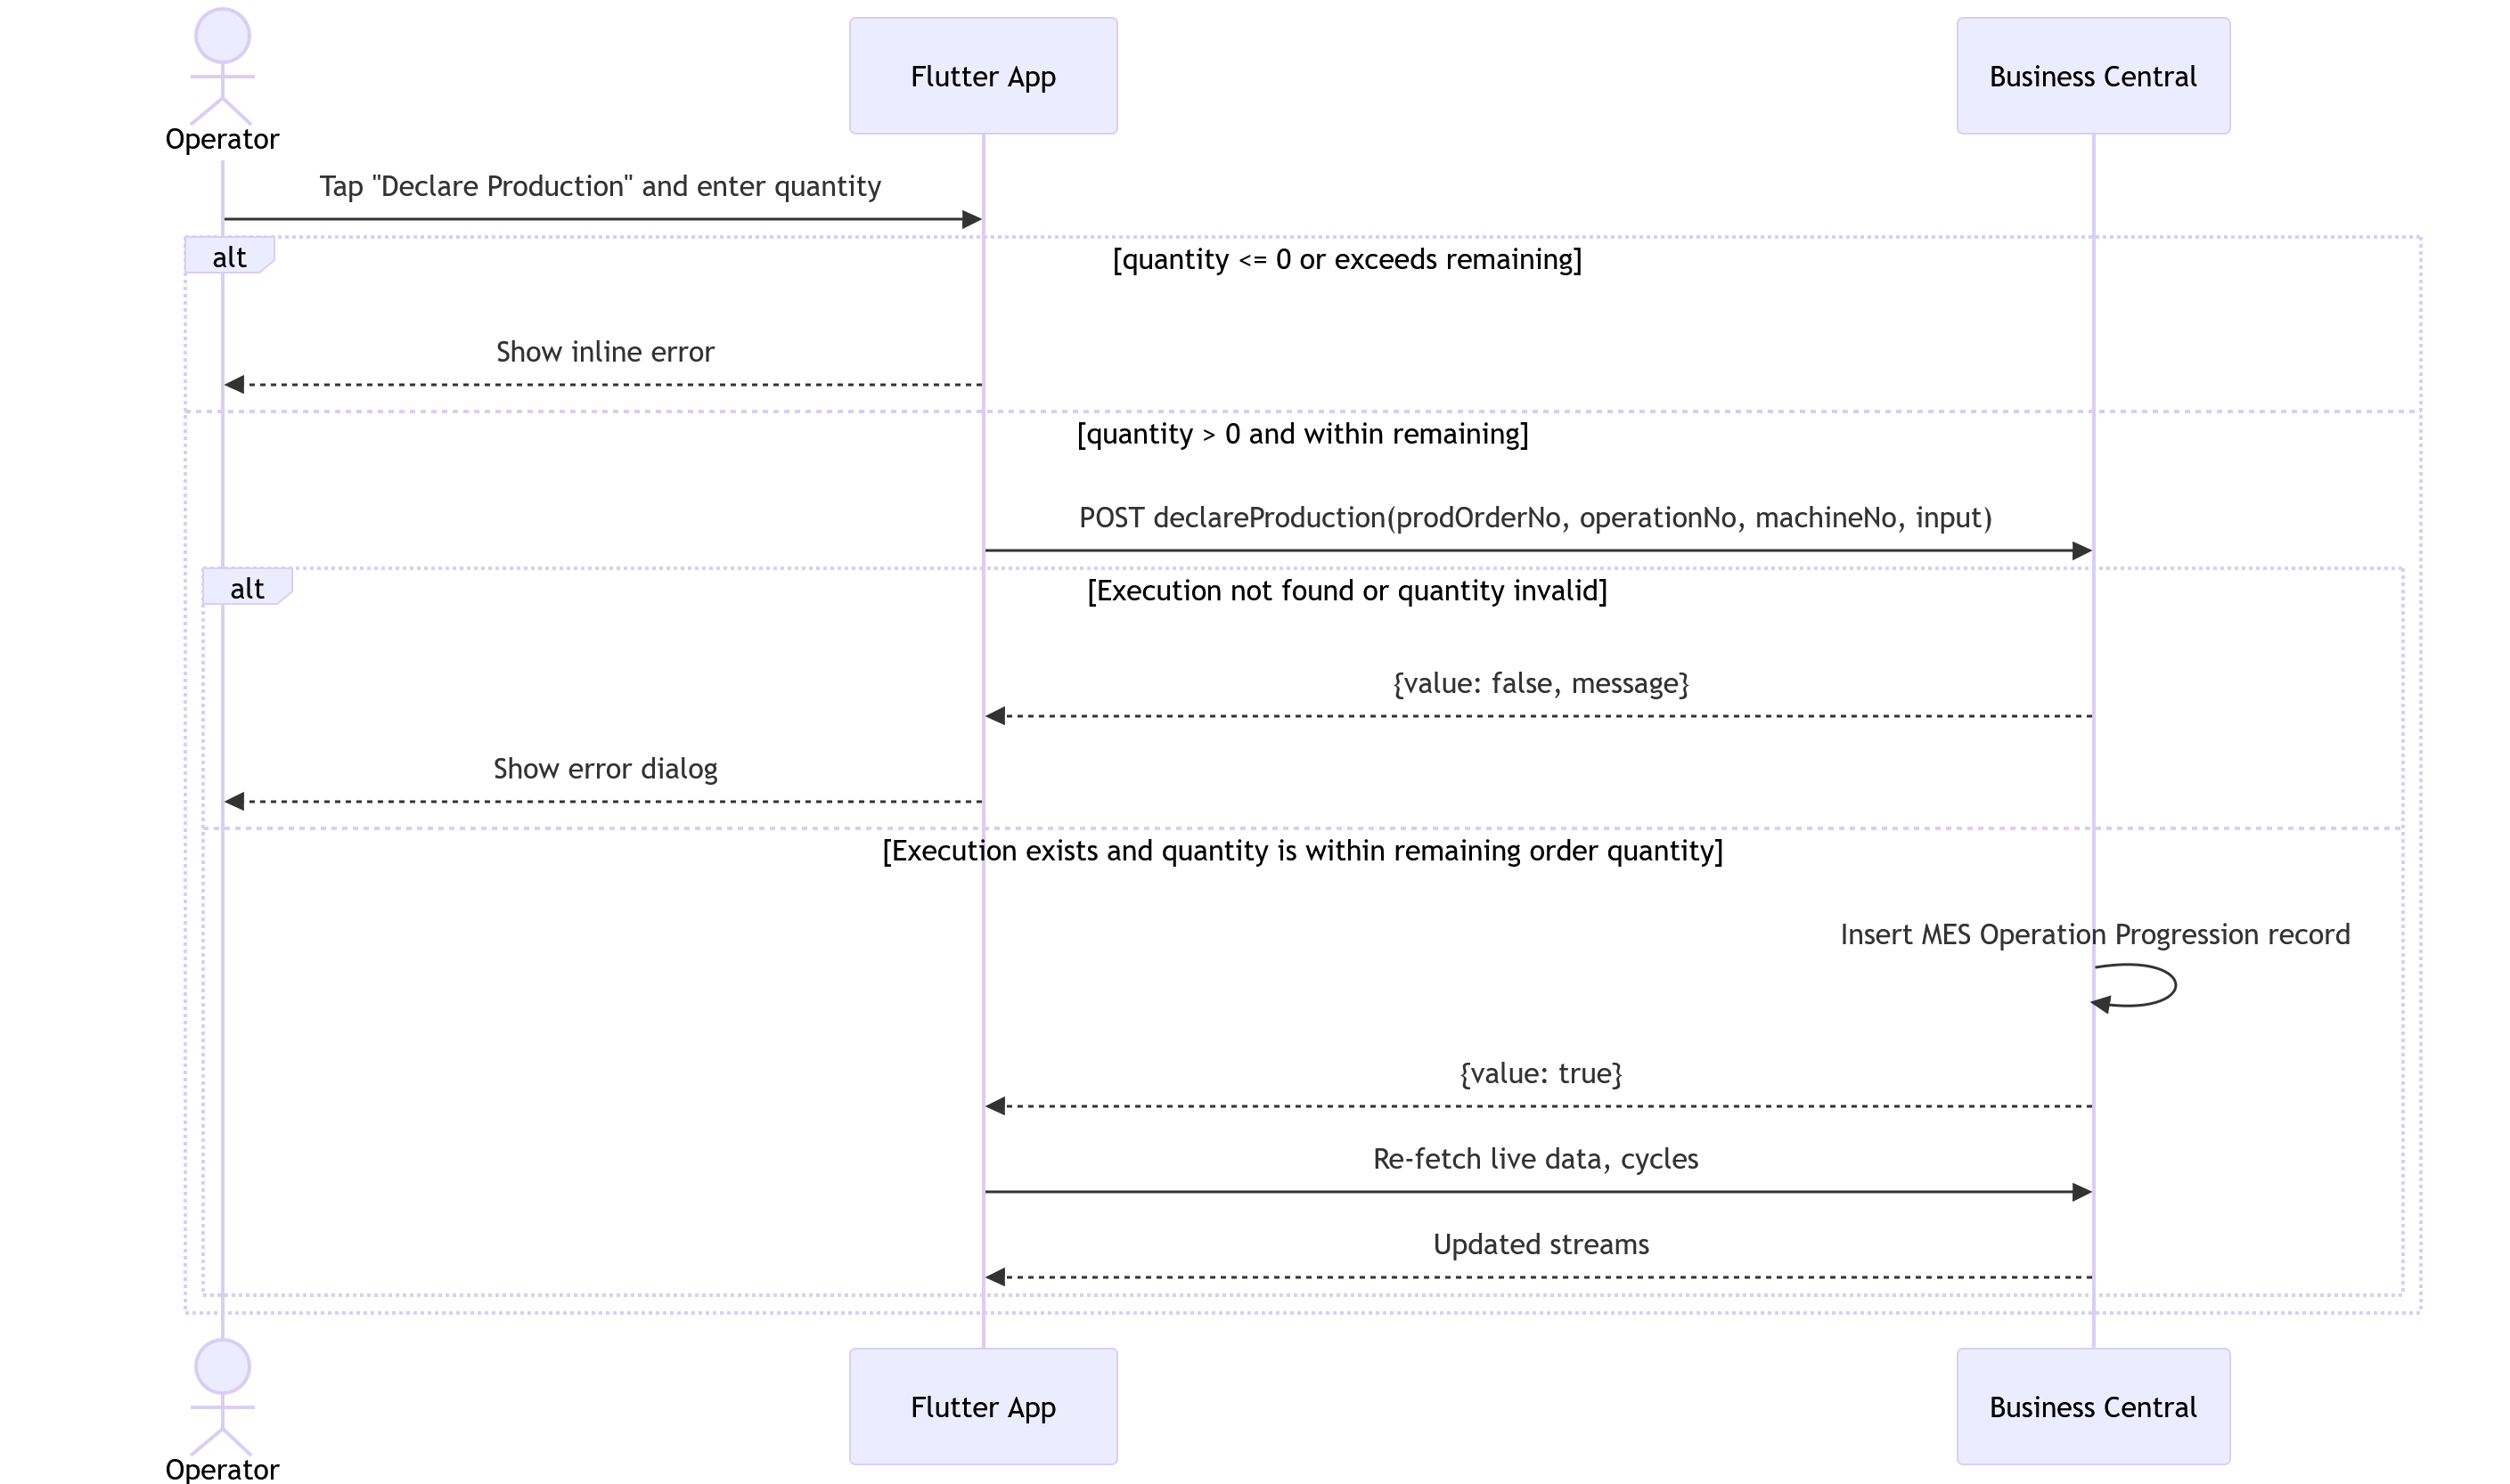
\includegraphics[width=\linewidth,height=0.82\textheight,keepaspectratio]{./media/MES_Sprint-3-Repport/diagrams/sequence/declare-production.png}
%   \caption{SD-12: Declare Production.}
%   \label{fig:s3-seq-declare-production}
% \end{figure}


%=====SD-12==========================================================
% sequenceDiagram
%     actor User
%     participant Flutter
%     participant Node as Node.js Middleware
%     participant AL
%     participant BC

%     rect rgb(220,235,255)
%         Note over User,BC: ref SD-01 — user is logged in and holds a valid token
%     end
%     rect rgb(220,235,255)
%         Note over User,BC: ref SD-11 — operation is in Running state, executionId known
%     end

%     User->>Flutter: Tap Declare Production → DeclareProductionDialog opens
%     opt Supervisor declaring on behalf of an operator
%         User->>Flutter: Select operator from OperatorSelector dropdown
%     end
%     User->>Flutter: Enter quantity, tap Submit
%     Flutter->>Flutter: Check component availability locally
%     alt Component availability check fails
%         Flutter-->>User: Show component error in dialog
%     else
%         Flutter->>Node: POST /api/declareProduction
%         Node->>AL: MESWebService_declareProduction
%         rect rgb(220,235,255)
%             Note over AL,BC: ref SD-02 — ValidateToken called, DeclaredById resolved from token
%         end
%         alt onBehalfOfUserId is set
%             AL->>BC: check that the user is a supervisor that has a shared departement with the operator
%         end
%         AL->>AL: set the operator id

%         AL->>BC: get the execution record of the operation
%         BC-->>AL: execution record 
%         AL->>BC: get the current progress of the execution
%         BC-->>AL: latest progression 
%         AL->>AL: validation
%         alt Validation failed or ExecutionId blank or No shared work center found
%             AL-->>Node: error response
%             Node-->>Flutter: error response
%             Flutter-->>User: Show error response
%         else Valid
%             AL->>BC: Insert MES Operation Progression
%             BC-->>AL: ok
%             AL-->>Node: success response
%             Node-->>Flutter: success response
%             Flutter->>Flutter: pops the dialog and refreshed the stream
%             Flutter-->>User: Navigate to Declaration Label Page
%         end
%     end
%====================================================================


Figures~\ref{fig:s3-seq-fetch-bom} and~\ref{fig:s3-seq-fetch-production-cycle}
present the two supplementary data-retrieval flows that run concurrently
alongside the main operation detail view. Both are polling streams that
re-emit on demand or when a state-change trigger is received from the
\techname{Flutter} client.
 
Figure~\ref{fig:s3-seq-fetch-bom} describes the bill-of-materials retrieval
flow. The \techname{AL} layer resolves the routing link code from the active
\domainterm{ProdOrderRoutingLine}, filters the production order components
by that link, aggregates the quantity already scanned per item, and resolves
per-unit quantities from the \domainterm{ItemUnitOfMeasure} table before
returning the assembled BOM rows to the \techname{Flutter} client.

\begin{figure}[H]
  \centering
  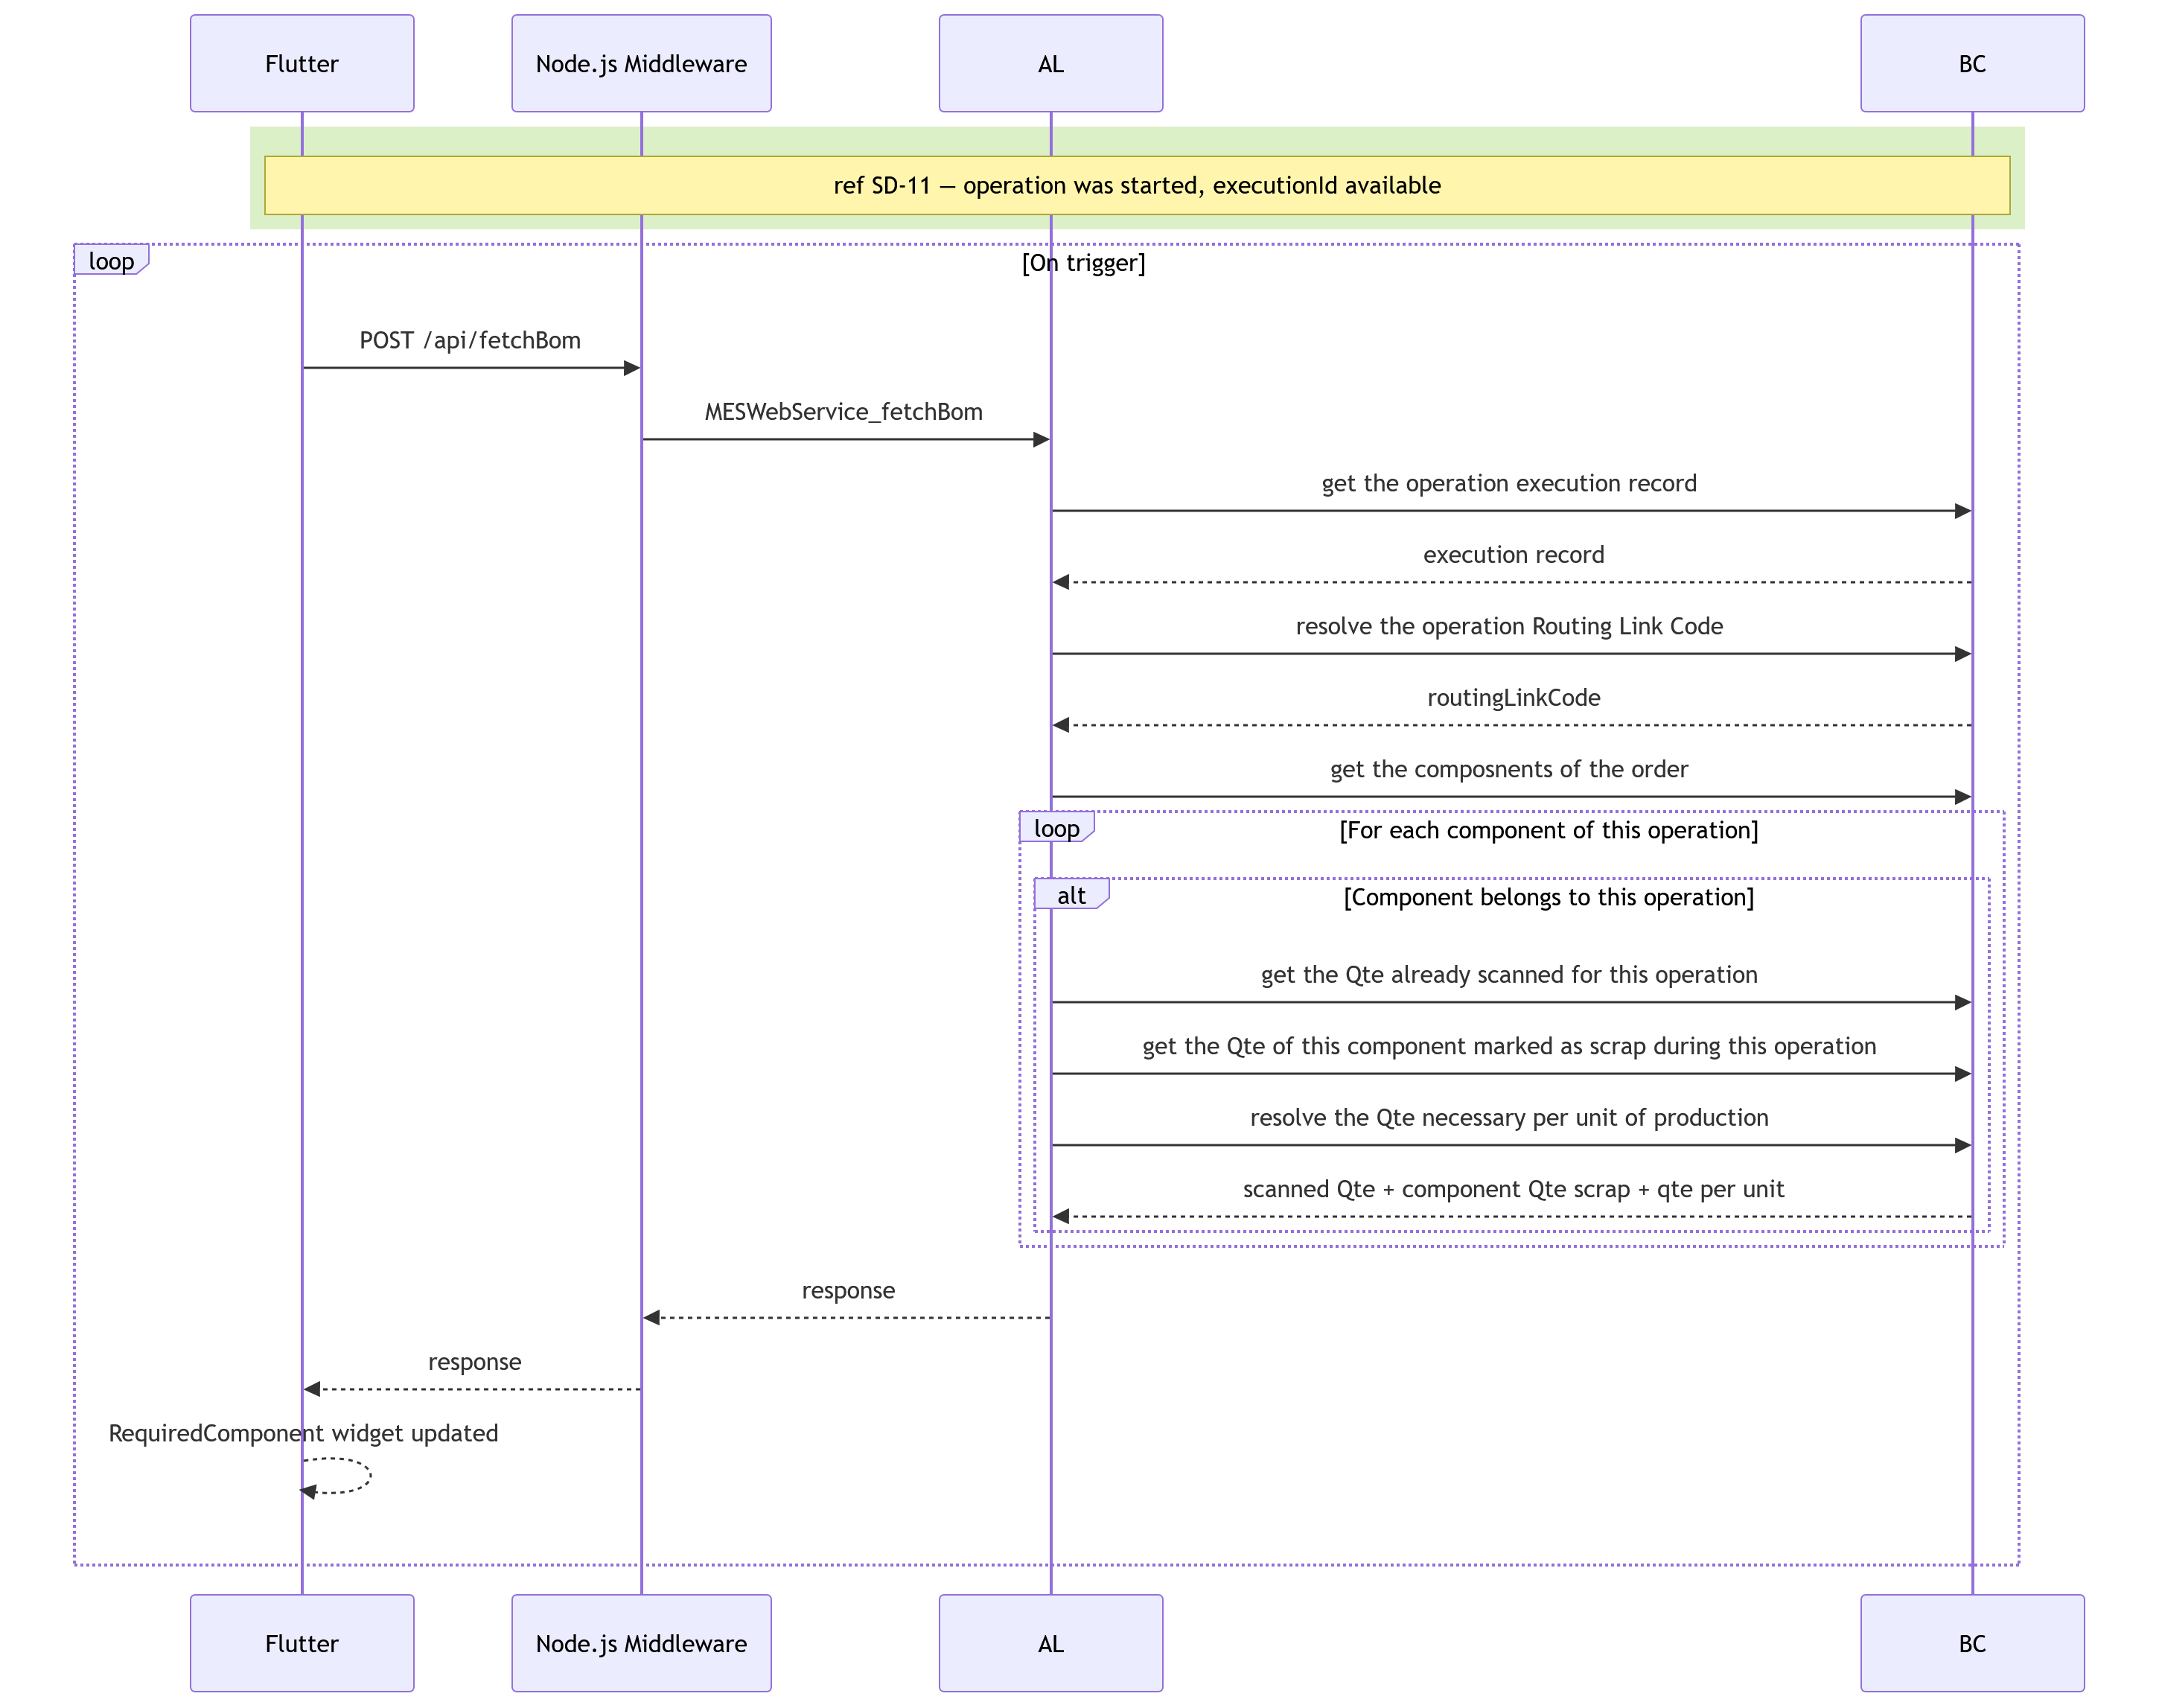
\includegraphics[width=\linewidth,height=0.82\textheight,keepaspectratio]{./media/MES_Sprint-3-Repport/diagrams/sequence/fetch-BOM.png}
  \caption{SD-21: Fetch Bill of Materials.}
  \label{fig:s3-seq-fetch-bom}
\end{figure}

%=====SD-21==========================================================
%  sequenceDiagram
%       participant Flutter
%       participant Node as Node.js Middleware
%       participant AL
%       participant BC

%       rect rgb(220,240,200)
%           Note over Flutter,BC: ref SD-11 — operation was started, executionId available
%       end

%       loop On trigger
%           Flutter->>Node: POST /api/fetchBom 
%           Node->>AL: MESWebService_fetchBom 

%           AL->>BC:get the operation execution record
%           BC-->>AL: execution record 
%           AL->>BC: resolve the operation Routing Link Code
%           BC-->>AL: routingLinkCode
%           AL->>BC: get the composnents of the order
%           loop For each component of this operation
%              alt Component belongs to this operation
%                   AL->>BC: get the Qte already scanned for this operation 
%                   AL->>BC: get the Qte of this component marked as scrap during this operation
%                   AL->>BC: resolve the Qte necessary per unit of production
%                   BC-->>AL: scanned Qte + component Qte scrap + qte per unit
%               end
%           end

%           AL-->>Node: response
%           Node-->>Flutter: response
%           Flutter-->>Flutter: RequiredComponent widget updated
%       end
%====================================================================

Figure~\ref{fig:s3-seq-fetch-production-cycle} illustrates the production-cycle
retrieval flow. The \techname{AL} layer fetches the full progression history
for the operation, enriches each entry with the name of the user who declared
it, and returns the assembled cycle list to the \techname{Flutter} client.

\begin{figure}[H]
  \centering
  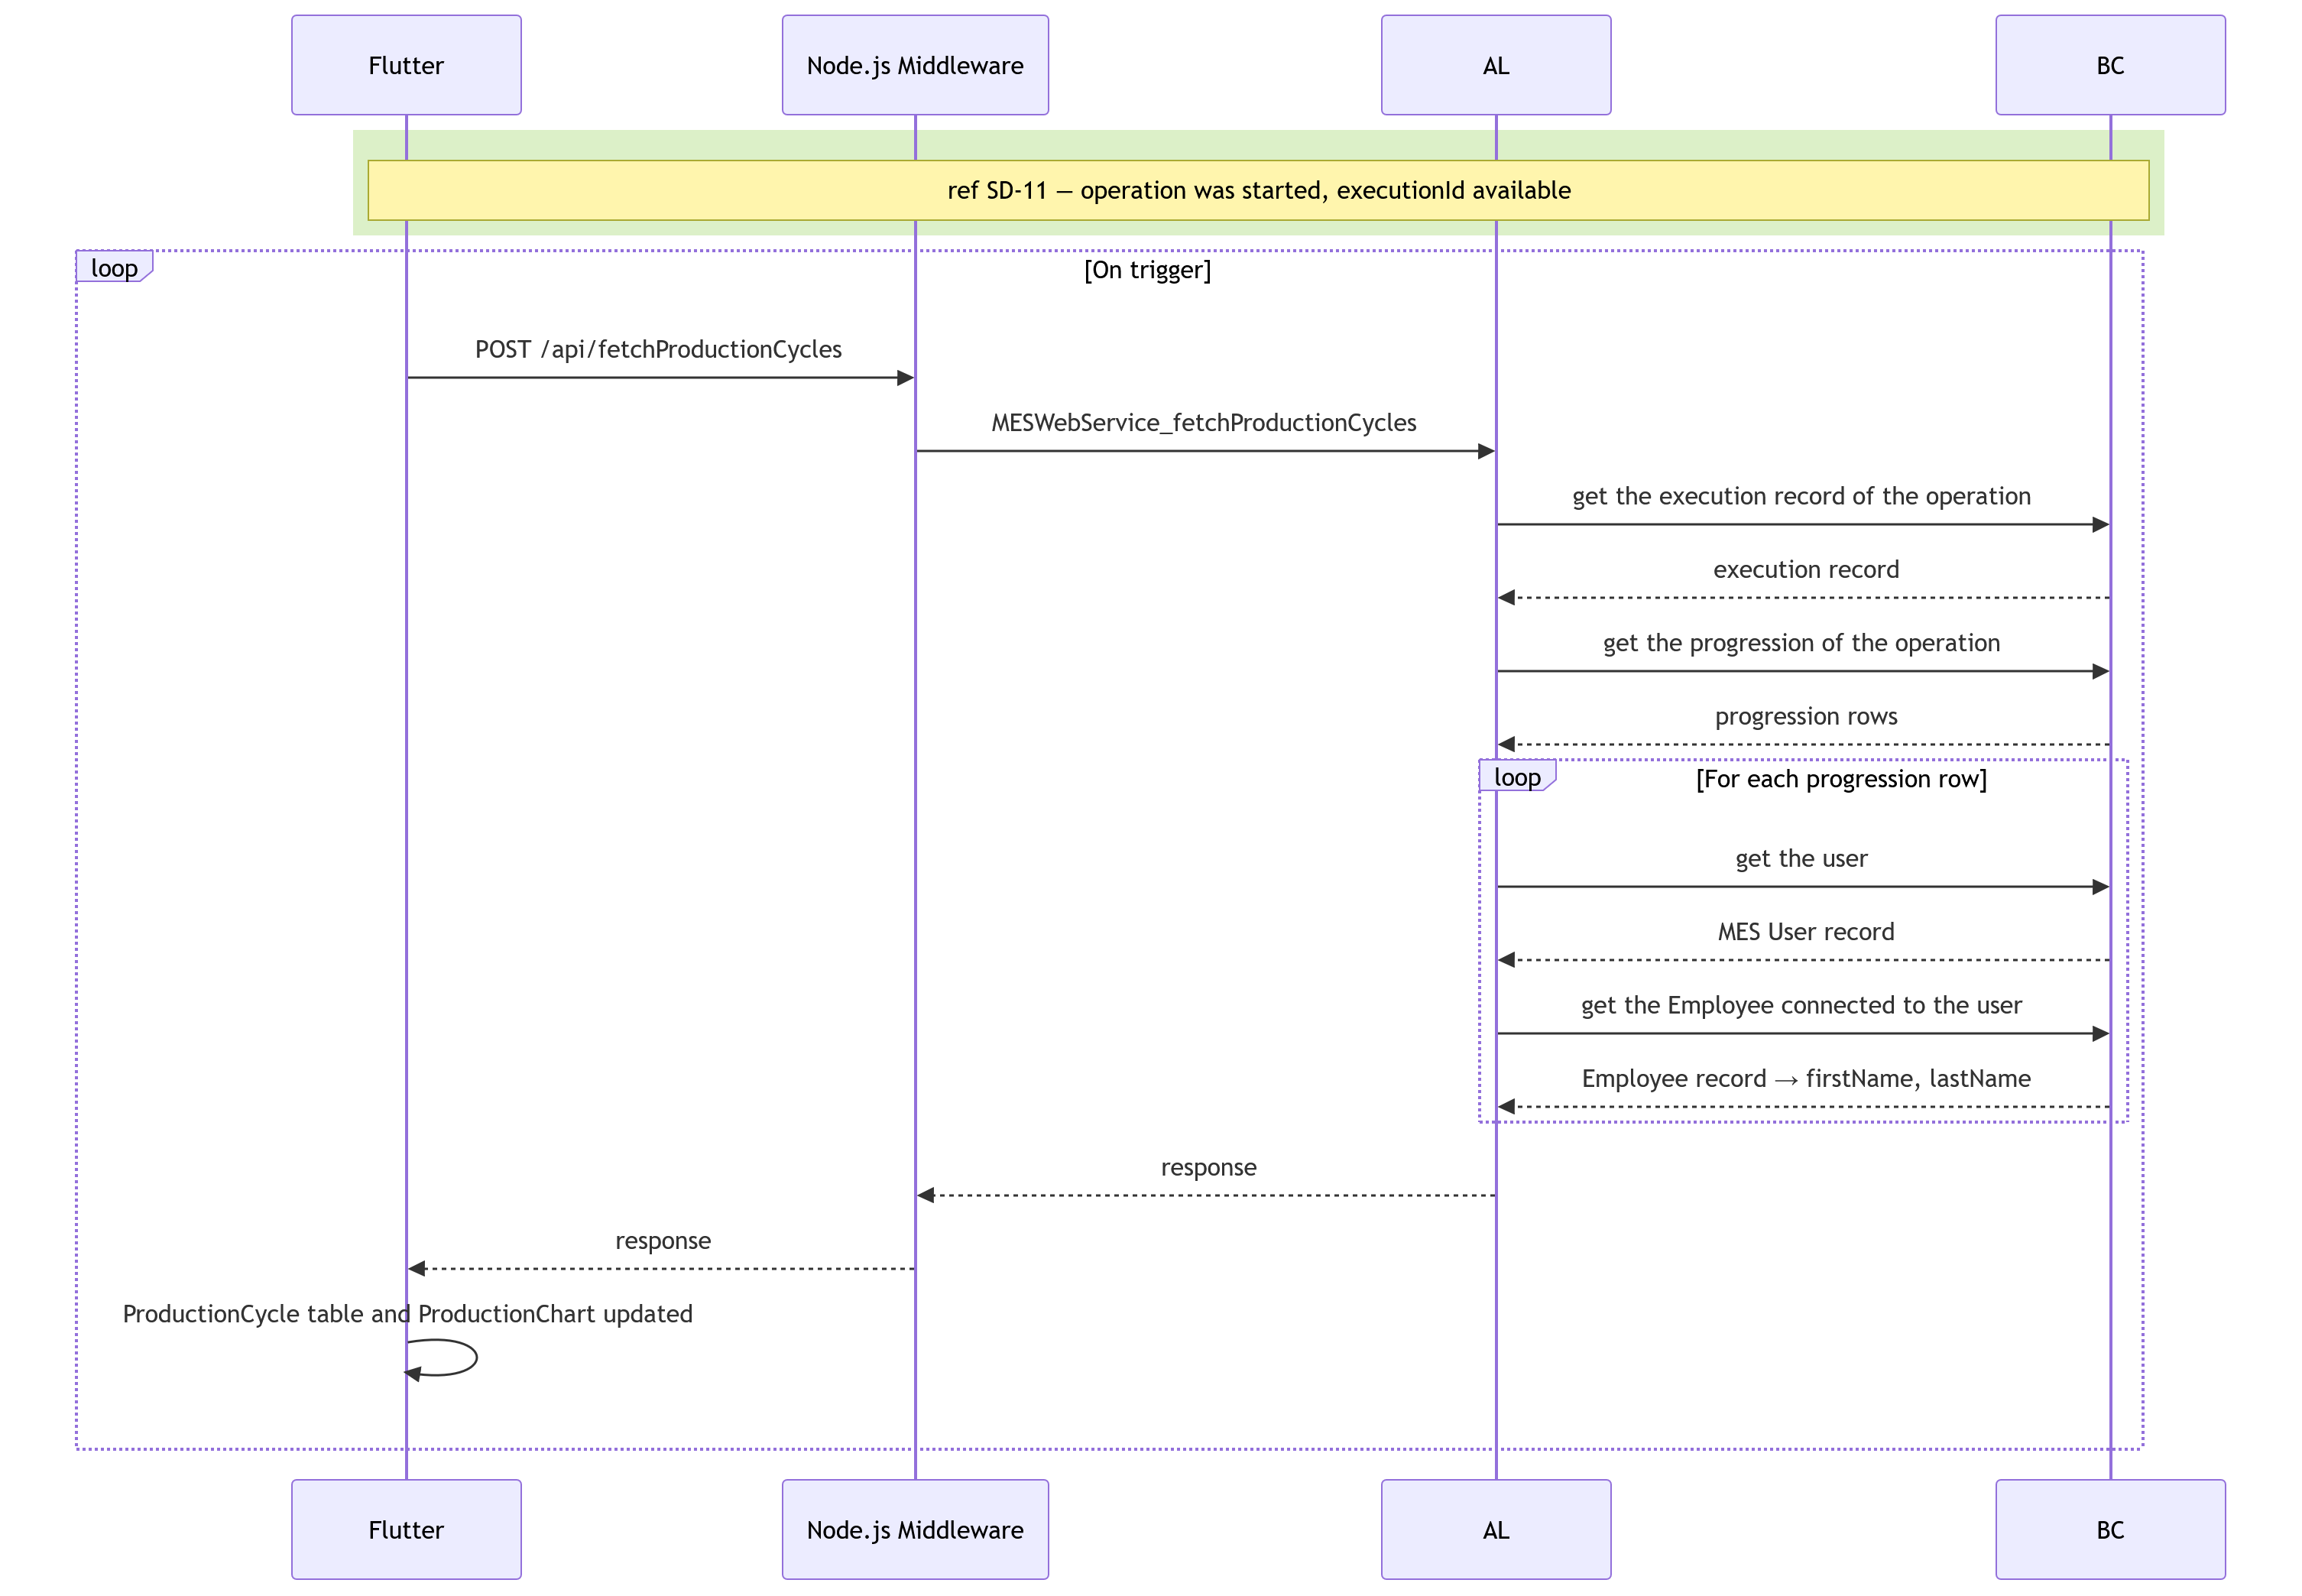
\includegraphics[width=\linewidth,height=0.82\textheight,keepaspectratio]{./media/MES_Sprint-3-Repport/diagrams/sequence/fetch-production-cycle.png}
  \caption{SD-22: Fetch Production Cycles.}
  \label{fig:s3-seq-fetch-production-cycle}
\end{figure}

%=====SD-22==========================================================
% sequenceDiagram
%       participant Flutter
%       participant Node as Node.js Middleware
%       participant AL
%       participant BC

%       rect rgb(220,240,200)
%           Note over Flutter,BC: ref SD-11 — operation was started, executionId available
%       end

%       loop On trigger
%           Flutter->>Node: POST /api/fetchProductionCycles 
%           Node->>AL: MESWebService_fetchProductionCycles 

%           AL->>BC: get the execution record of the operation
%           BC-->>AL: execution record 
%           AL->>BC: get the progression of the operation
%           BC-->>AL: progression rows

%           loop For each progression row
%               AL->>BC: get the user
%               BC-->>AL: MES User record
%               AL->>BC: get the Employee connected to the user
%               BC-->>AL: Employee record → firstName, lastName
%           end

%           AL-->>Node: response
%           Node-->>Flutter: response
%           Flutter->>Flutter: ProductionCycle table and ProductionChart updated
%       end
%====================================================================

Figures~\ref{fig:s3-seq-pause-operation} through~\ref{fig:s3-seq-resume-operation}
illustrate the operation: pause, resume. Figure~\ref{fig:s3-seq-pause-operation} describes the pause flow. The
\techname{AL} layer confirms that the operation is currently in the
\domainterm{Running} state before inserting a \domainterm{Paused}
\domainterm{MES Operation State} record and setting the machine status
back to \domainterm{Idle}.

\begin{figure}[H]
  \centering
  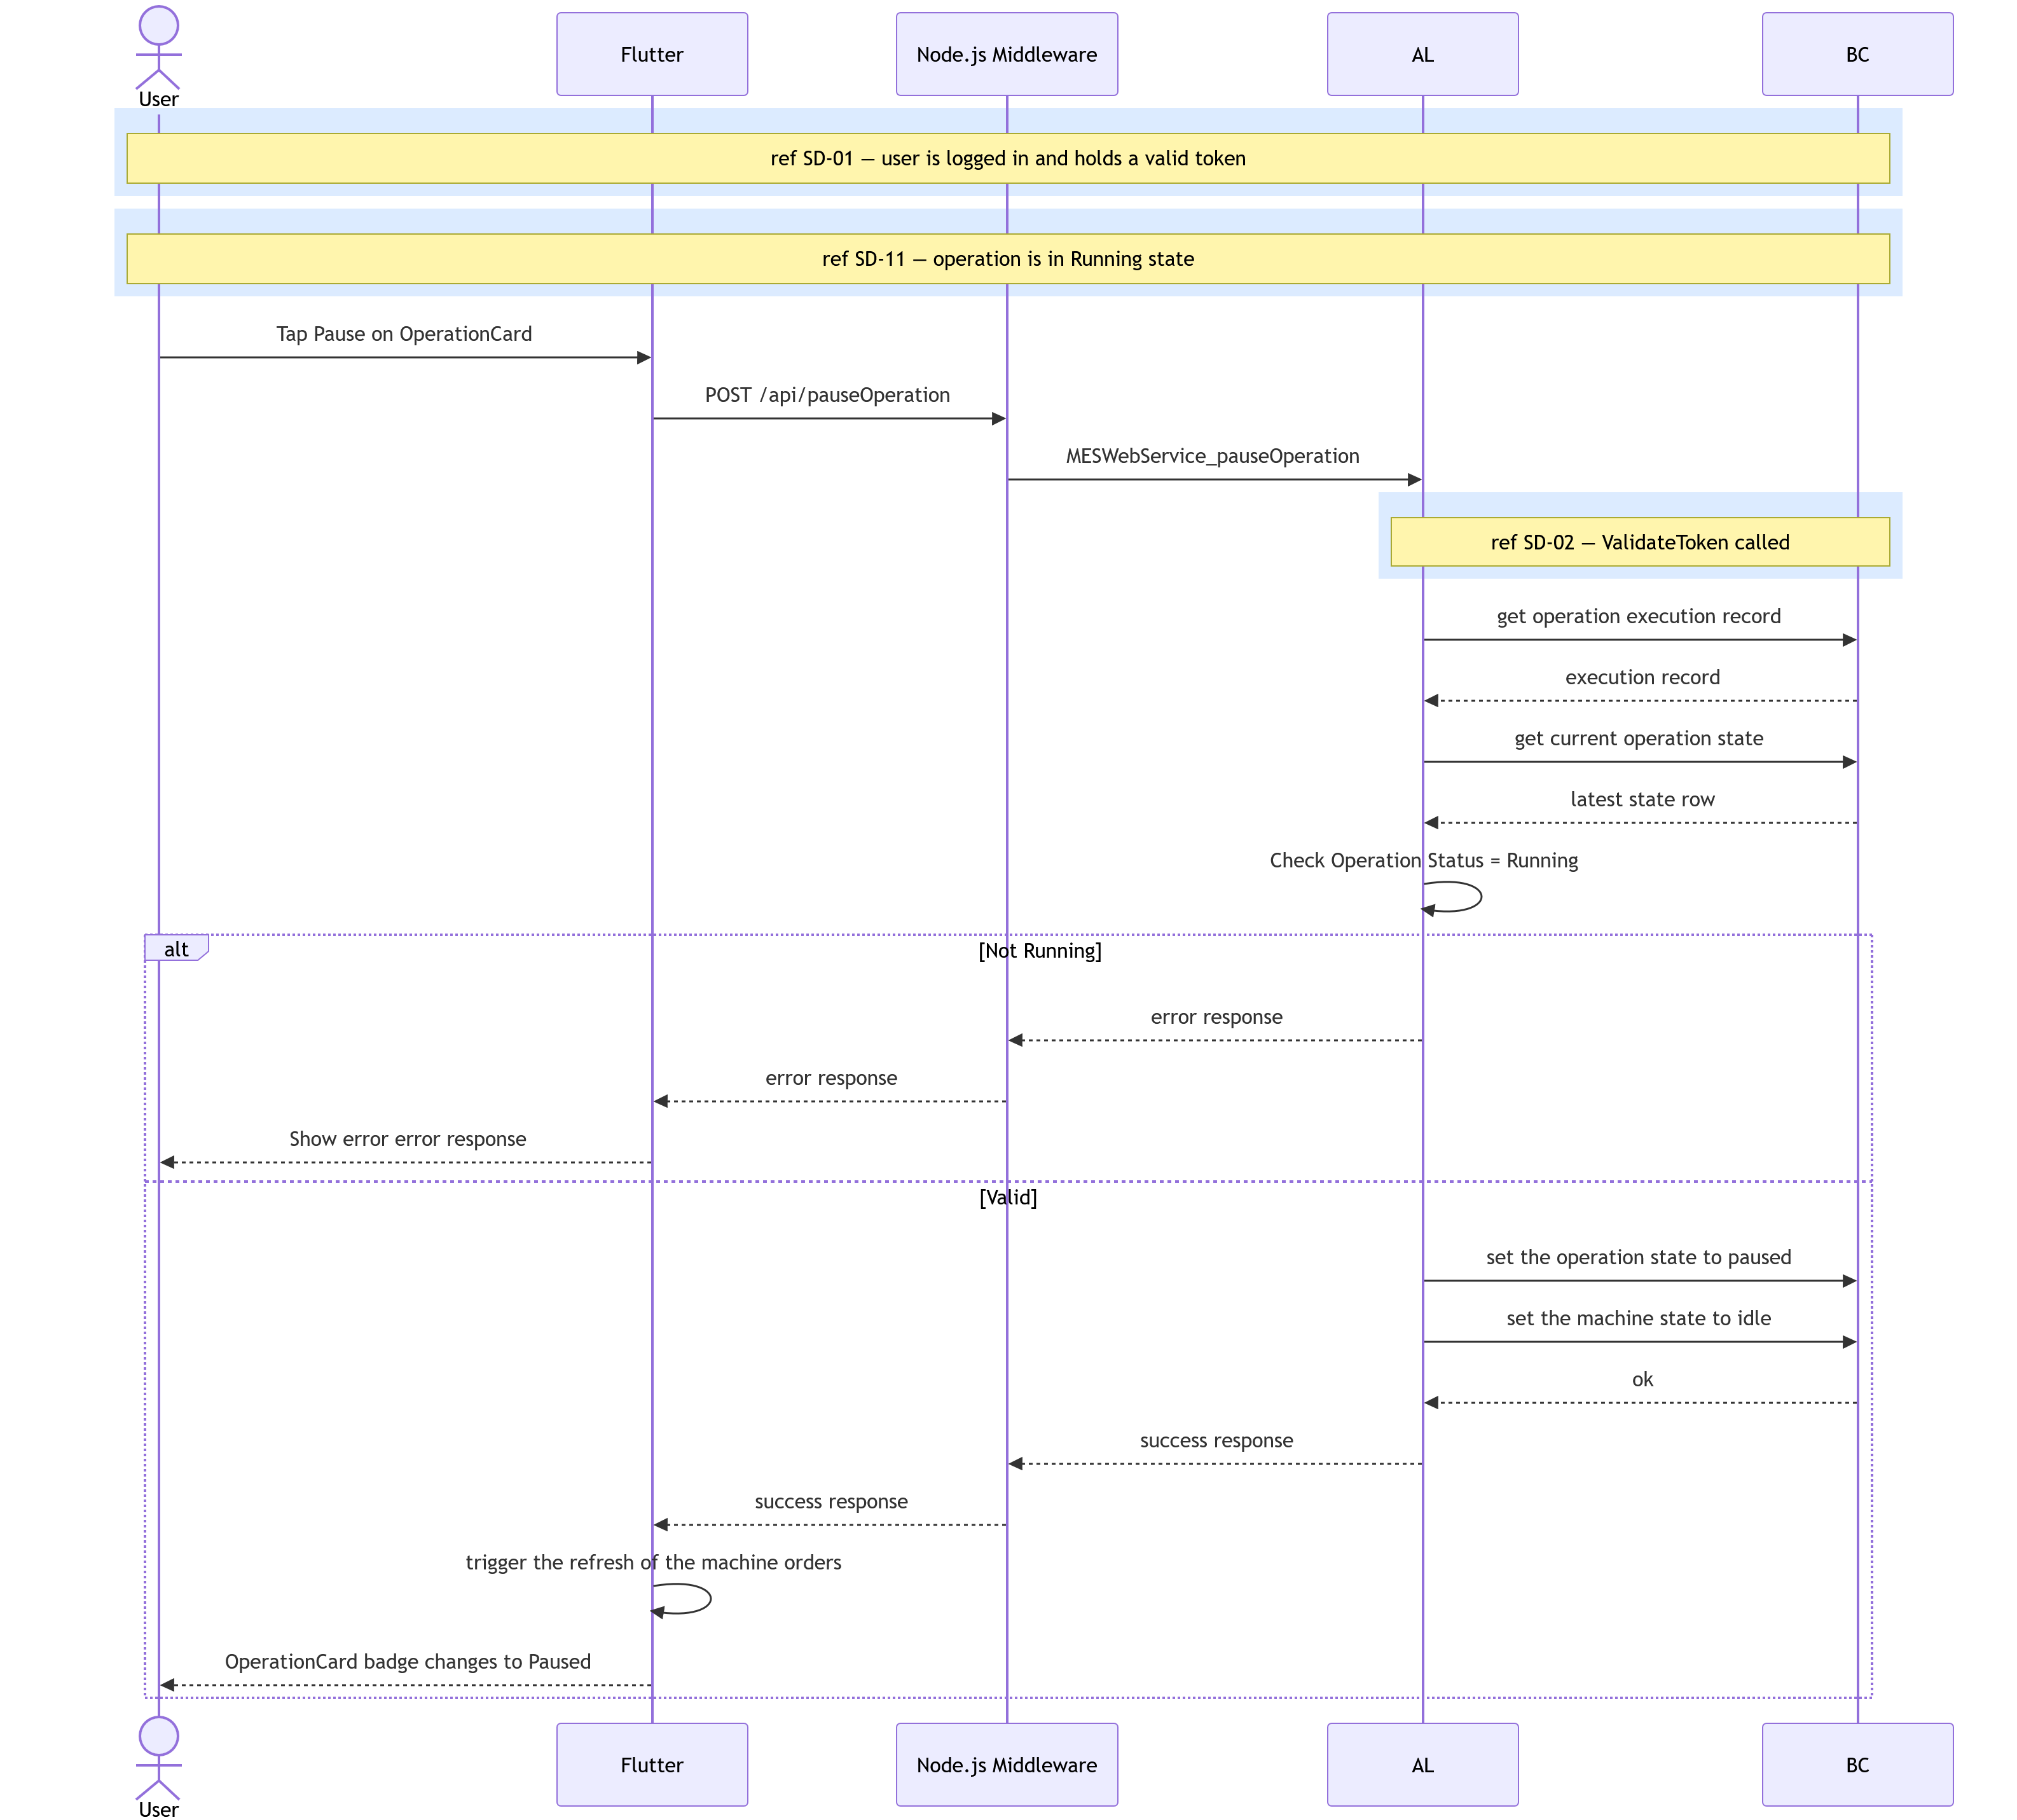
\includegraphics[width=\linewidth,height=0.82\textheight,keepaspectratio]{./media/MES_Sprint-3-Repport/diagrams/sequence/pause-operation.png}
  \caption{SD-13: Pause Operation.}
  \label{fig:s3-seq-pause-operation}
\end{figure}

%=====SD-13==========================================================
% sequenceDiagram
%       actor User
%       participant Flutter
%       participant Node as Node.js Middleware
%       participant AL
%       participant BC

%       rect rgb(220,235,255)
%           Note over User,BC: ref SD-01 — user is logged in and holds a valid token
%       end
%       rect rgb(220,235,255)
%           Note over User,BC: ref SD-11 — operation is in Running state
%       end

%       User->>Flutter: Tap Pause on OperationCard
%       Flutter->>Node: POST /api/pauseOperation
%       Node->>AL: MESWebService_pauseOperation 

%       rect rgb(220,235,255)
%           Note over AL,BC: ref SD-02 — ValidateToken called
%       end

%       AL->>BC: get operation execution record
%       BC-->>AL: execution record 
%       AL->>BC: get current operation state 
%       BC-->>AL: latest state row
%       AL->>AL: Check Operation Status = Running
%       alt Not Running
%           AL-->>Node: error response
%           Node-->>Flutter: error response
%           Flutter-->>User: Show error error response
%       else Valid
%           AL->>BC: set the operation state to paused
%           AL->>BC: set the machine state to idle
%           BC-->>AL: ok
%           AL-->>Node: success response
%           Node-->>Flutter: success response
%           Flutter->>Flutter: trigger the refresh of the machine orders
%           Flutter-->>User: OperationCard badge changes to Paused
%       end
%====================================================================

Figure~\ref{fig:s3-seq-resume-operation} presents the resume flow. In addition
to confirming that the operation is in the \domainterm{Paused} state, the
\techname{AL} layer verifies that no other operation is currently running on
the same machine before inserting a \domainterm{Running} state record and
marking the machine as \domainterm{Working}.

\begin{figure}[H]
  \centering
  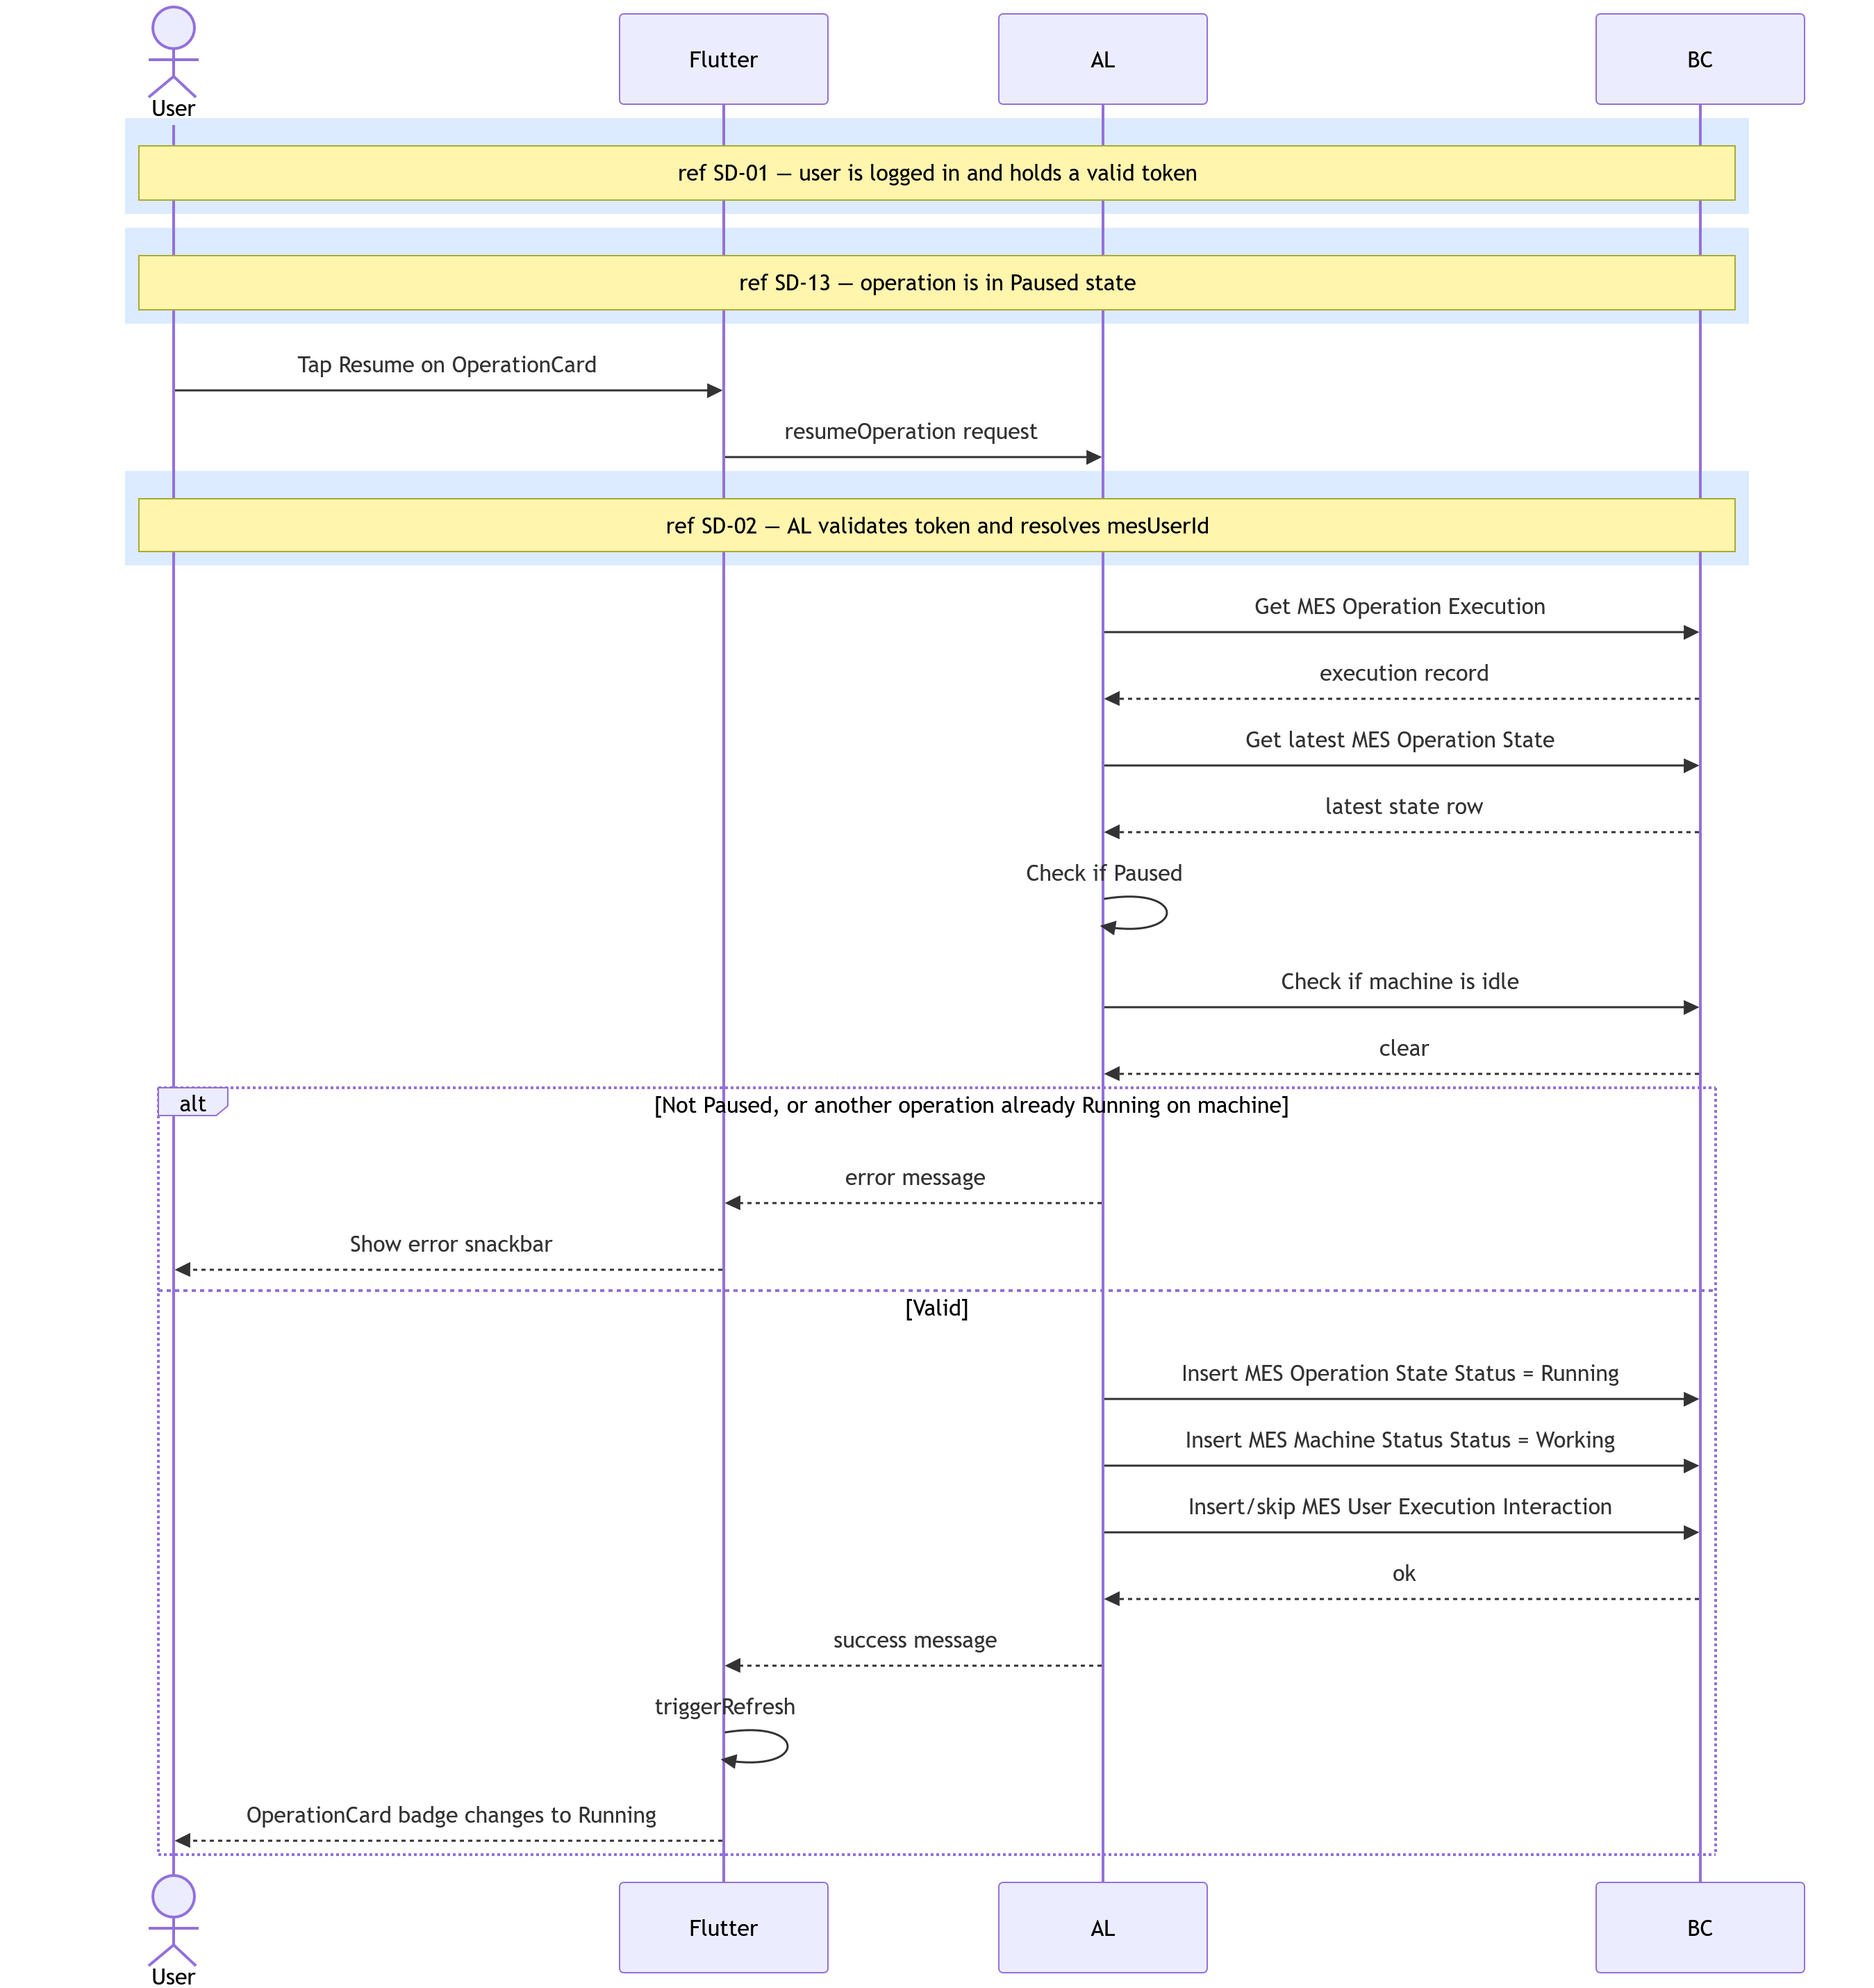
\includegraphics[width=\linewidth,height=0.82\textheight,keepaspectratio]{./media/MES_Sprint-3-Repport/diagrams/sequence/resume-operation.png}
  \caption{SD-14: Resume Operation.}
  \label{fig:s3-seq-resume-operation}
\end{figure}

%=====SD-14==========================================================
% sequenceDiagram
%       actor User
%       participant Flutter
%       participant Node as Node.js Middleware
%       participant AL
%       participant BC

%       rect rgb(220,235,255)
%           Note over User,BC: ref SD-01 — user is logged in and holds a valid token
%       end
%       rect rgb(220,235,255)
%           Note over User,BC: ref SD-13 — operation is in Paused state
%       end

%       User->>Flutter: Tap Resume on OperationCard
%       Flutter->>Node: POST /api/resumeOperation 
%       Node->>AL: MESWebService_resumeOperation 

%       rect rgb(220,235,255)
%           Note over AL,BC: ref SD-02 — ValidateToken called
%       end

%       AL->>BC: get the execution record of the operation
%       BC-->>AL: execution record 
%       AL->>BC: get the state of the operation
%       BC-->>AL: latest state row
%       AL->>AL: check if the operation is Paused
%       AL->>BC: check if the machine is idle
%       BC-->>AL: clear
%       alt Another operation is Running on machine or Not Paused
%           AL-->>Node: error response
%           Node-->>Flutter: error response
%           Flutter-->>User: Show error response
%       else Valid
%           AL->>BC: set the operation to running
%           AL->>BC: set machine to working
%           BC-->>AL: ok
%           AL-->>Node: success response
%           Node-->>Flutter: success response
%           Flutter->>Flutter: trigger refresh
%           Flutter-->>User: OperationCard badge updates
%       end
%====================================================================

Figure~\ref{fig:s3-seq-finish_cancel_interupt-operation} covers the finish and cancel
flows, which share a single endpoint family. The \techname{AL} layer rejects
the request if the operation is already in a terminal state; otherwise it
inserts the appropriate closed-state record, stamps the execution end time,
and resets the machine status to \domainterm{Idle}. The closed operation then
appears in the history view rather than the active operations list.	

\begin{figure}[H]
  \centering
  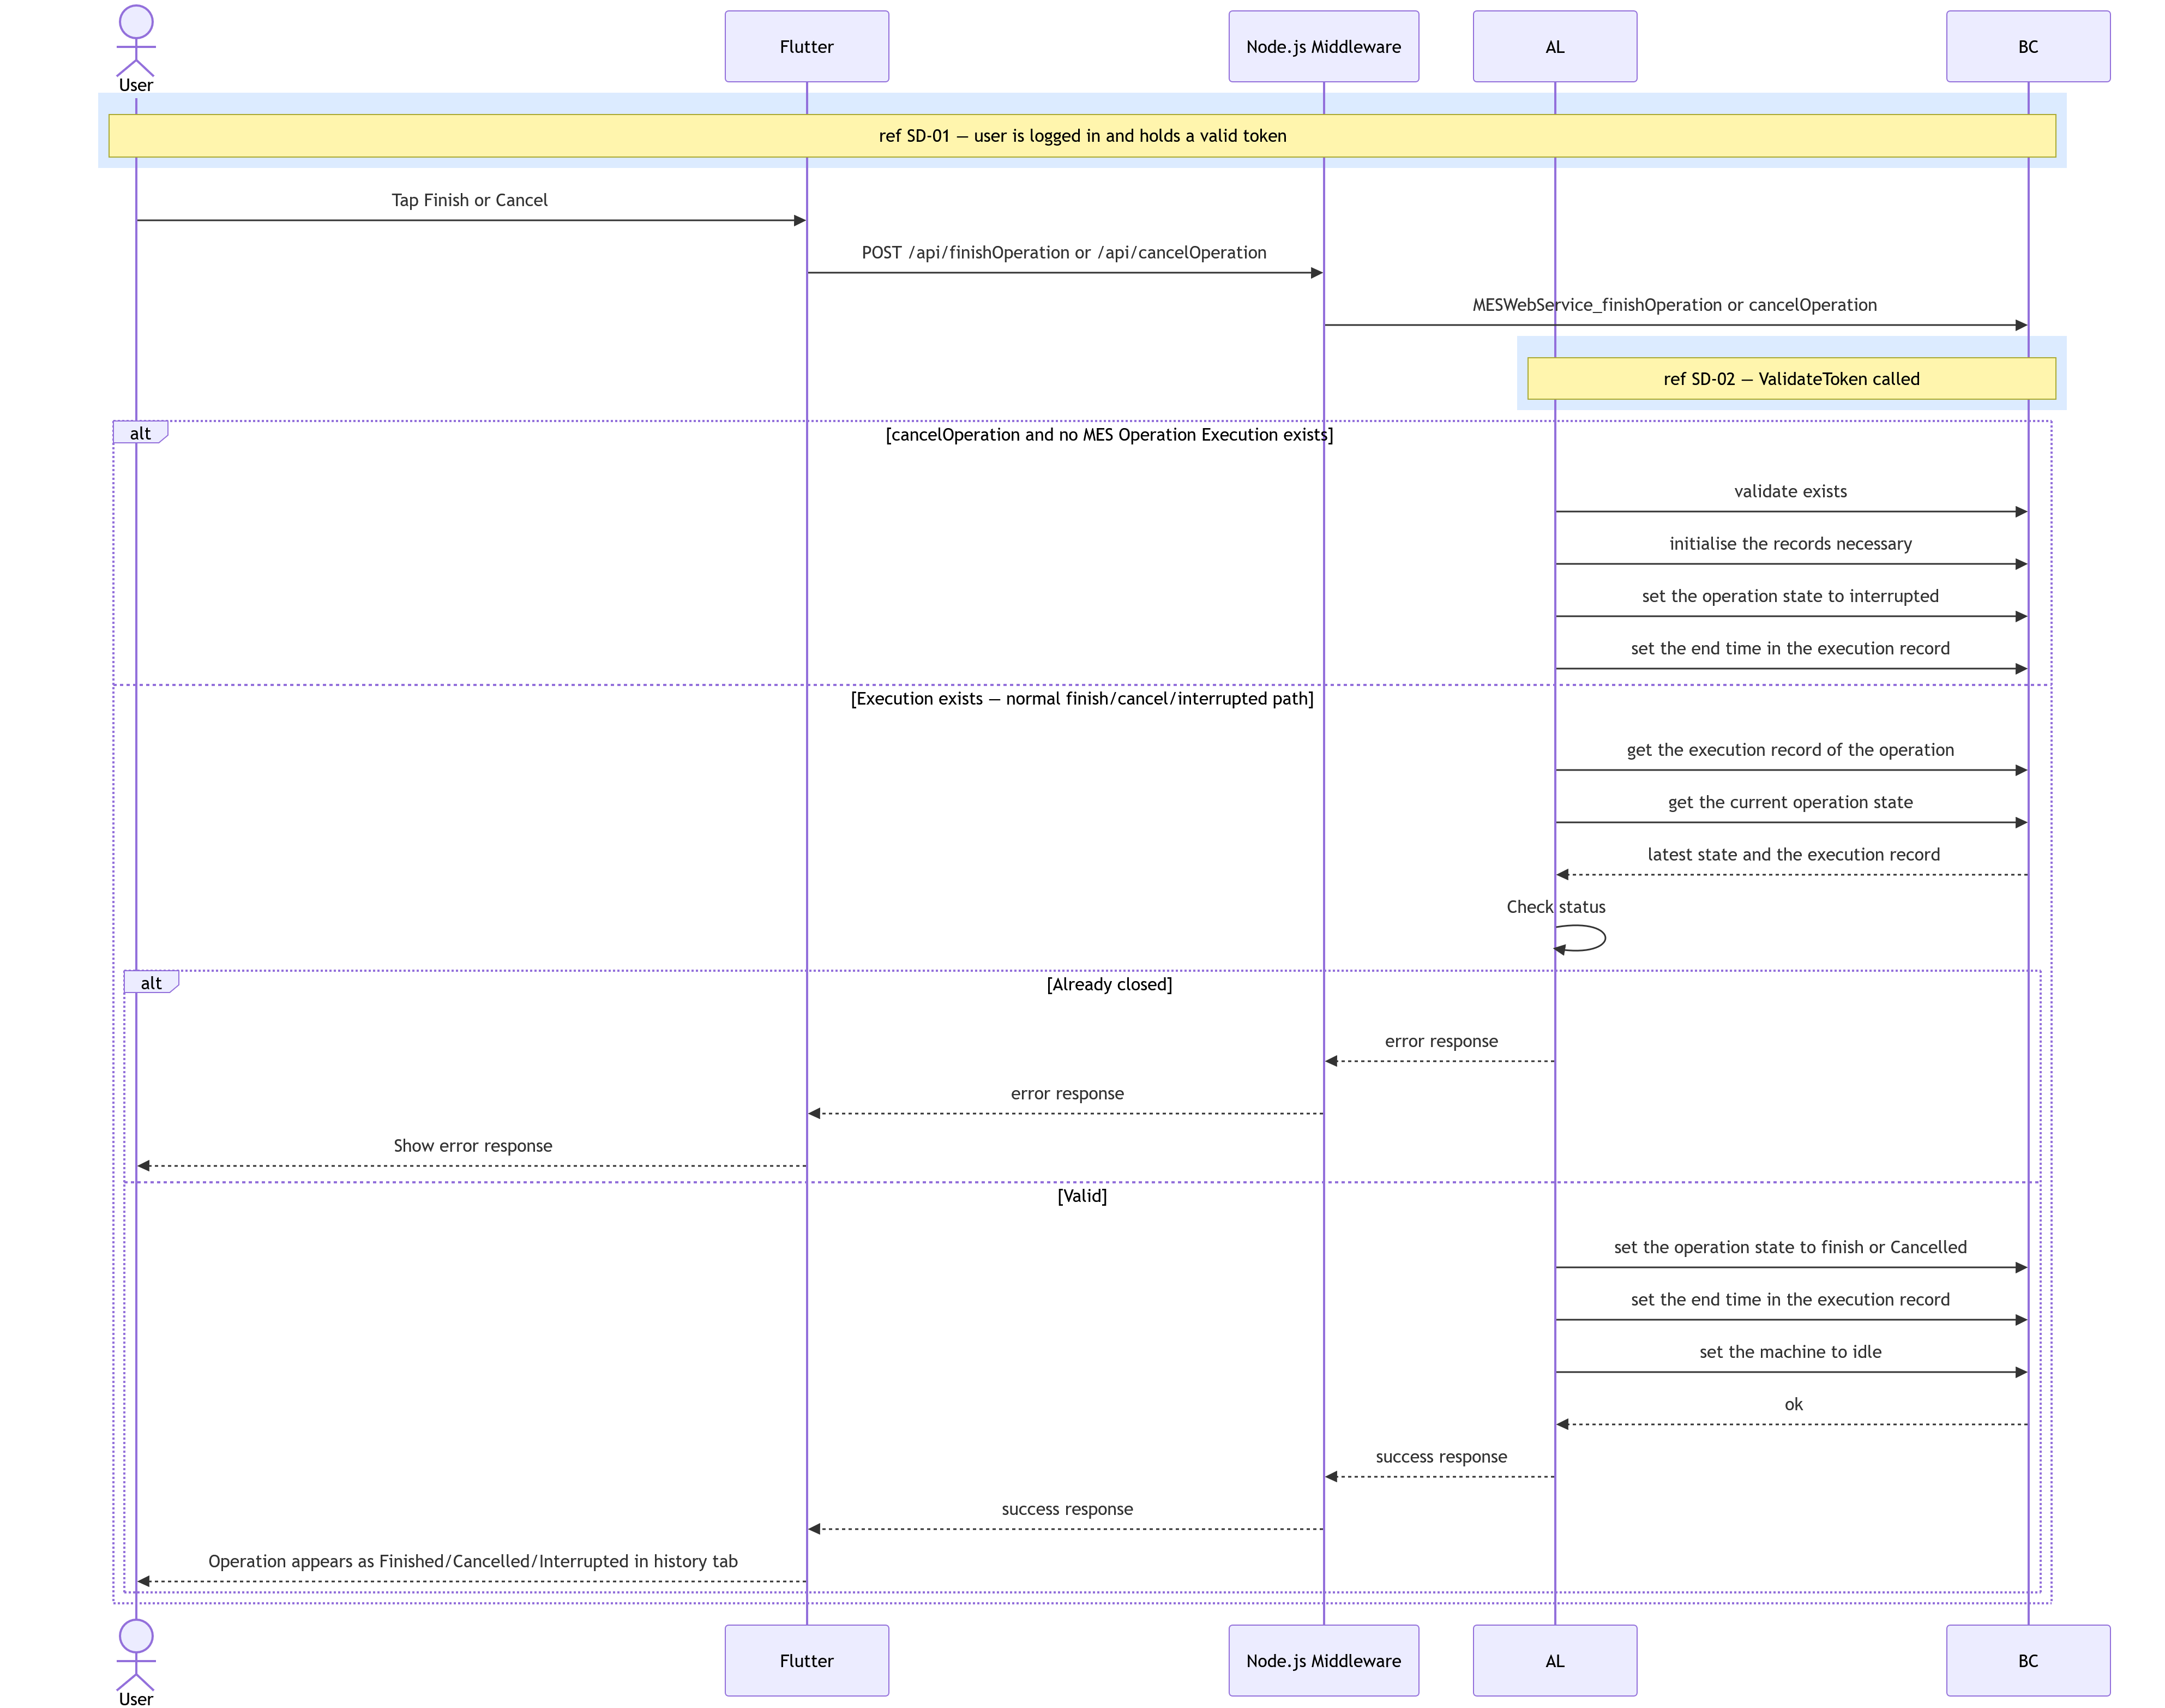
\includegraphics[width=\linewidth,height=0.82\textheight,keepaspectratio]{./media/MES_Sprint-3-Repport/diagrams/sequence/finish_cancel_interrupt-operation.png}
  \caption{SD-15: Finish/Cancel/Interrupt Operation.}
  \label{fig:s3-seq-finish_cancel_interupt-operation}
\end{figure}

%=====SD-15==========================================================
% sequenceDiagram
%     actor User
%     participant Flutter
%     participant AL
%     participant BC

%     rect rgb(220,235,255)
%         Note over User,BC: ref SD-01 — user is logged in and holds a valid token
%     end
%     rect rgb(220,235,255)
%         Note over User,BC: ref SD-11 — operation was started (Running or Paused)
%     end

%     User->>Flutter: Tap Finish (or Cancel)
%     Flutter->>AL: finishOperation or cancelOperation request

%     rect rgb(220,235,255)
%         Note over User,BC: ref SD-02 — AL validates token and resolves mesUserId
%     end

%     AL->>BC: Get MES Operation Execution
%     BC-->>AL: execution record
%     AL->>BC: Get latest MES Operation State
%     BC-->>AL: latest state
%     AL->>AL: Check if Finished or Cancelled
%     alt Already closed
%         AL-->>Flutter: error message
%         Flutter-->>User: Show error snackbar
%     else Valid
%         AL->>BC: Insert MES Operation State Status = Finished/Cancelled
%         AL->>BC: Update MES Operation Execution — set EndTime = now
%         AL->>BC: Insert MES Machine Status Status = Idle
%         AL->>BC: Insert/skip MES User Execution Interaction
%         BC-->>AL: ok
%         AL-->>Flutter: success message
%         Flutter-->>User: Operation appears as Finished/Cancelled in history
%     end
%====================================================================

% Figure~\ref{fig:s3-seq-declare-scrap} describes the scrap declaration flow.
% Before inserting the scrap record, the \techname{AL} layer verifies that
% the operation has not already been finished, cancelled, or paused, and that
% the referenced scrap code exists in \techname{Business Central}. On success,
% it inserts a \domainterm{MES Operation Scrap} entry, records user interaction,
% and appends a new \domainterm{MES Operation Progression} row so that the
% scrap quantity is reflected in the live data stream.

% \begin{figure}[H]
%   \centering
%   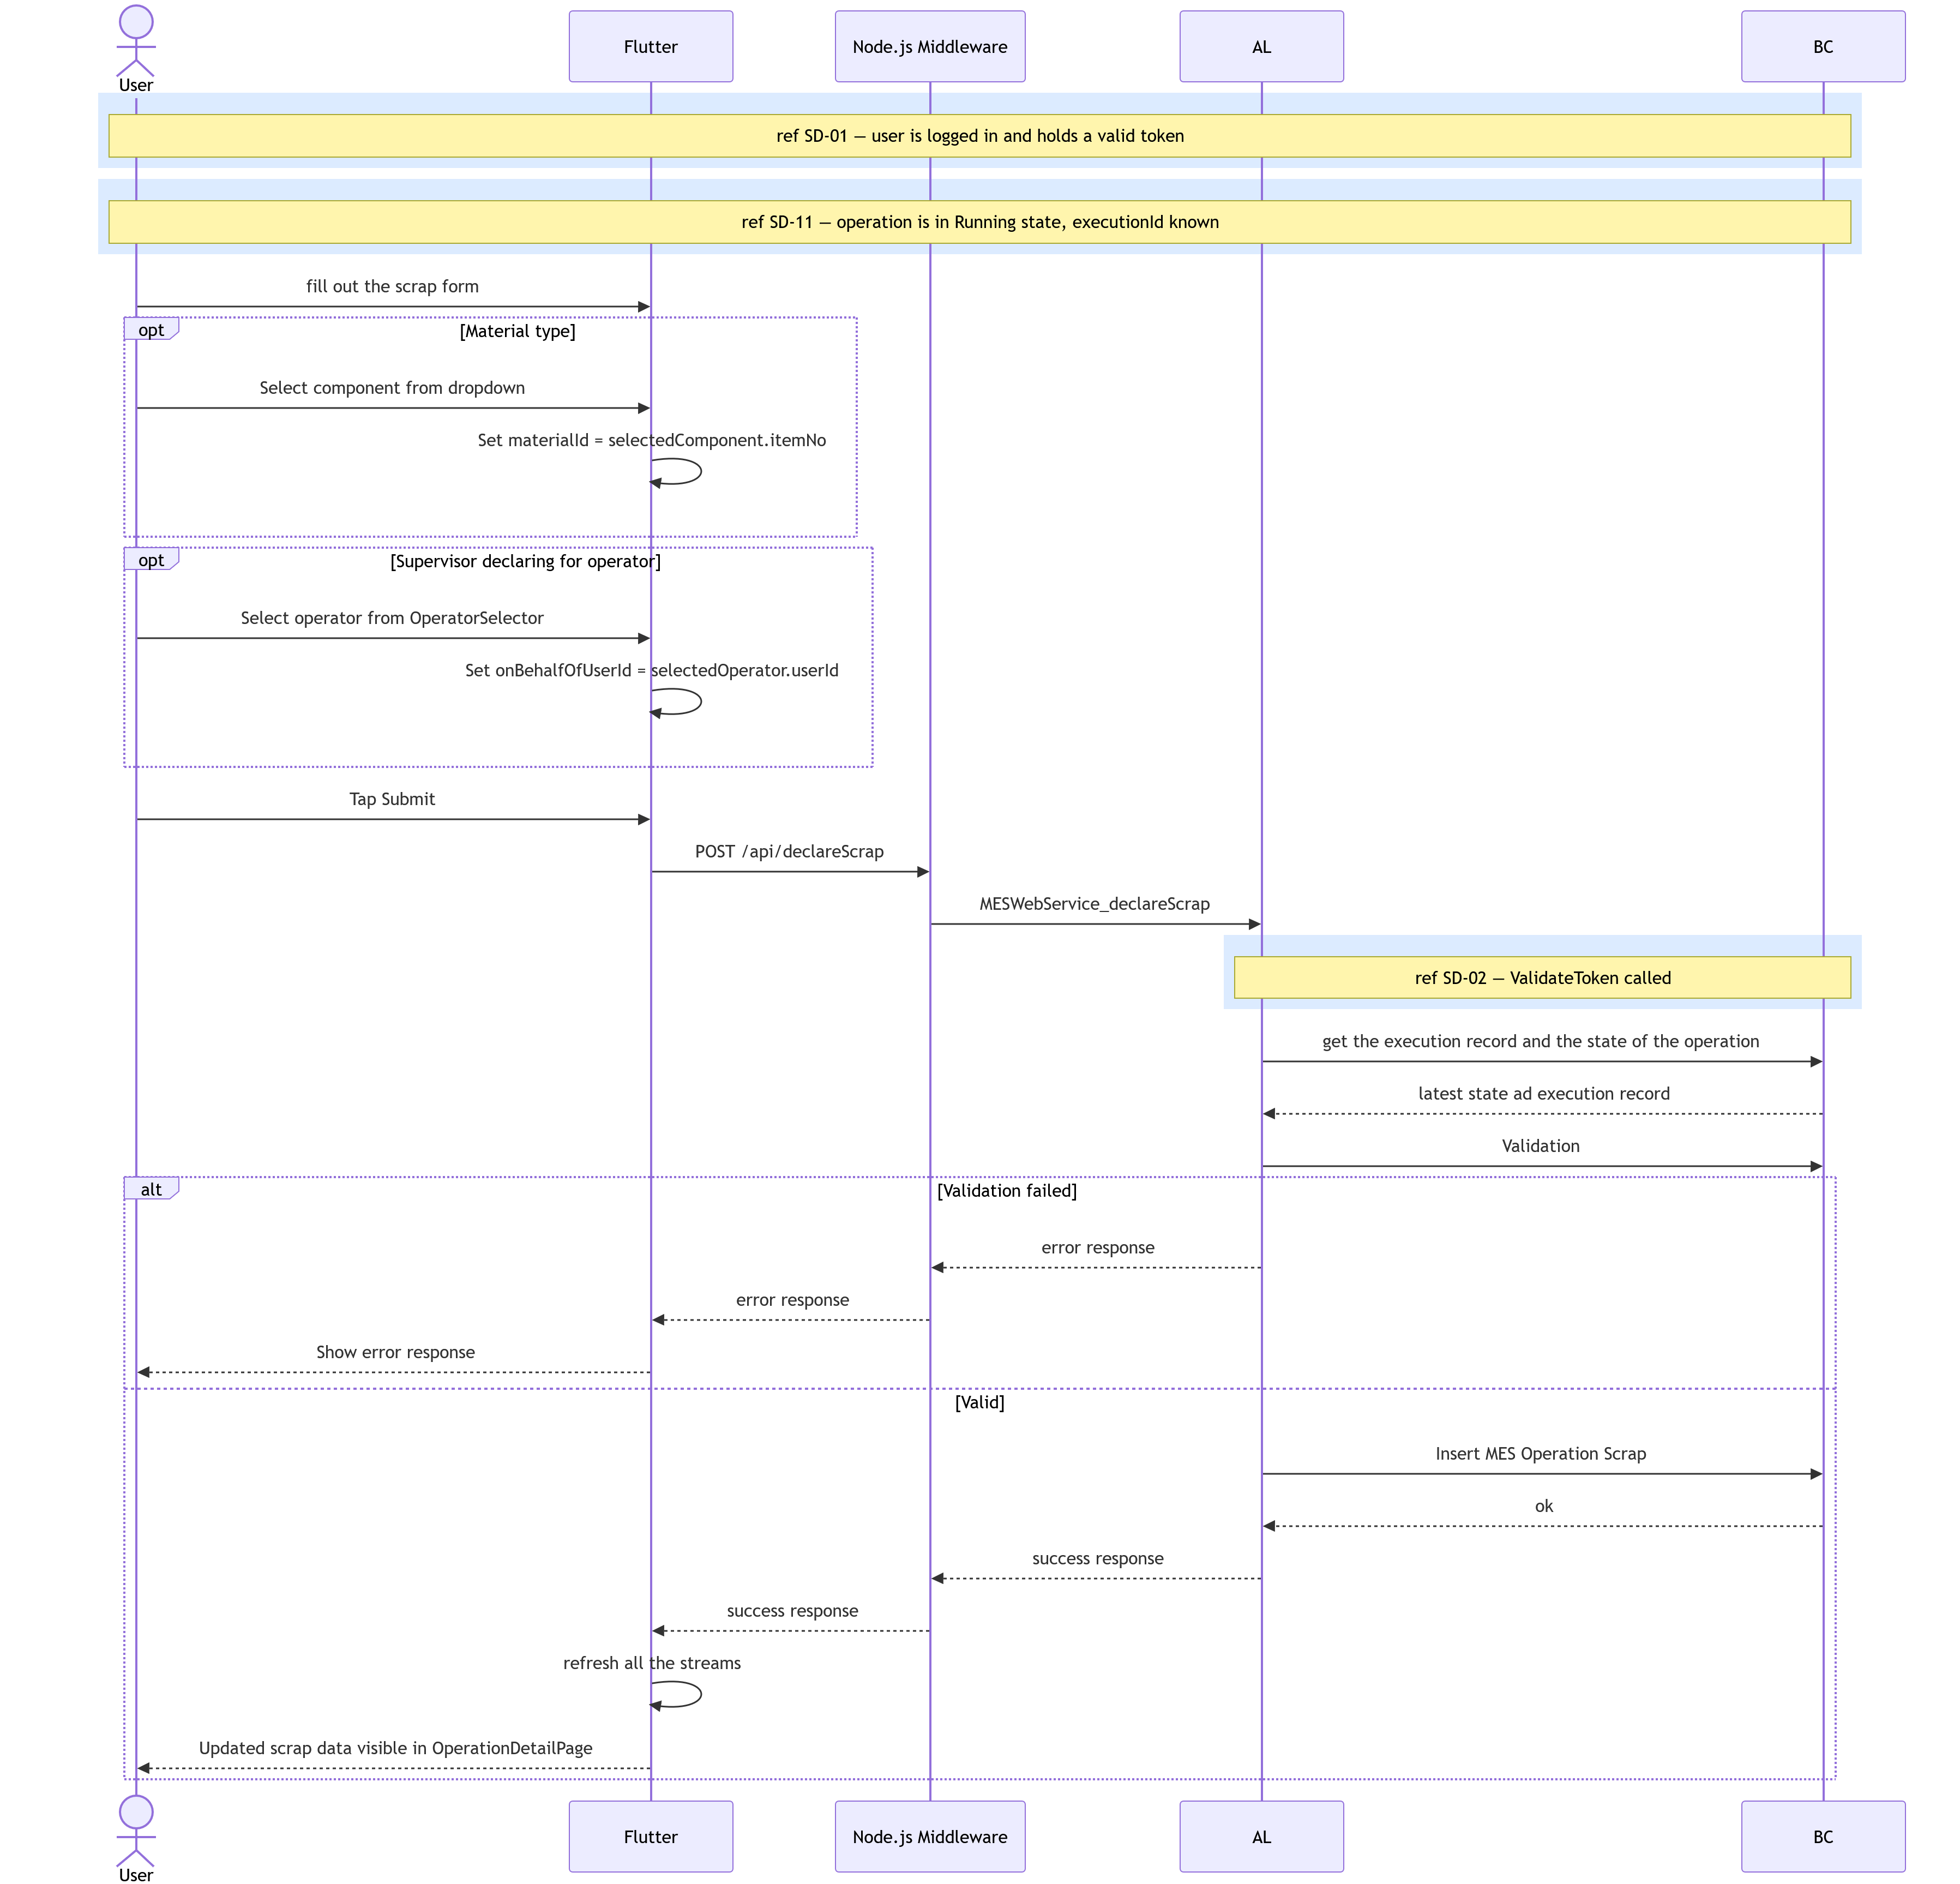
\includegraphics[width=\linewidth,height=0.82\textheight,keepaspectratio]{./media/MES_Sprint-3-Repport/diagrams/sequence/declare-scrap.png}
%   \caption{SD-16: declare scrap.}
%   \label{fig:s3-seq-declare-scrap}
% \end{figure}

%=====SD-16==========================================================
% sequenceDiagram
%     actor User
%     participant Flutter
%     participant Node as Node.js Middleware
%     participant AL
%     participant BC

%     rect rgb(220,235,255)
%         Note over User,BC: ref SD-01 — user is logged in and holds a valid token
%     end
%     rect rgb(220,235,255)
%         Note over User,BC: ref SD-11 — operation is in Running state, executionId known
%     end
%     User->>Flutter: fill out the scrap form
%     opt Material type
%         User->>Flutter: Select component from dropdown
%         Flutter->>Flutter: Set materialId = selectedComponent.itemNo
%     end
%     opt Supervisor declaring for operator
%         User->>Flutter: Select operator from OperatorSelector
%         Flutter->>Flutter: Set onBehalfOfUserId = selectedOperator.userId
%     end
%     User->>Flutter: Tap Submit
%     Flutter->>Node: POST /api/declareScrap
%     Node->>AL: MESWebService_declareScrap 

%       rect rgb(220,235,255)
%           Note over AL,BC: ref SD-02 — ValidateToken called
%       end

%       AL->>BC: get the execution record and the state of the operation
%       BC-->>AL: latest state ad execution record
%       AL->>BC: Validation
%       alt Validation failed
%           AL-->>Node: error response
%           Node-->>Flutter: error response
%           Flutter-->>User: Show error response
%       else Valid
%           AL->>BC: Insert MES Operation Scrap
%           BC-->>AL: ok
%           AL-->>Node: success response
%           Node-->>Flutter: success response
%           Flutter->>Flutter: refresh all the streams
%           Flutter-->>User: Updated scrap data visible in OperationDetailPage
%       end
%====================================================================

% Figure~\ref{fig:s3-seq-scan-component} illustrates the component scanning flow,
% which operates in two steps. First, the \techname{Flutter} client resolves
% each scanned barcode into an item record via a lightweight \texttt{resolveBarcode}
% call and accumulates the results locally. Once the operator confirms the
% batch, a single \texttt{insertScans} request is sent to the \techname{AL}
% layer, which inserts one \domainterm{MES Component Consumption} record per
% scanned item and records the associated user interaction entries.

% \begin{figure}[H]
%   \centering
%   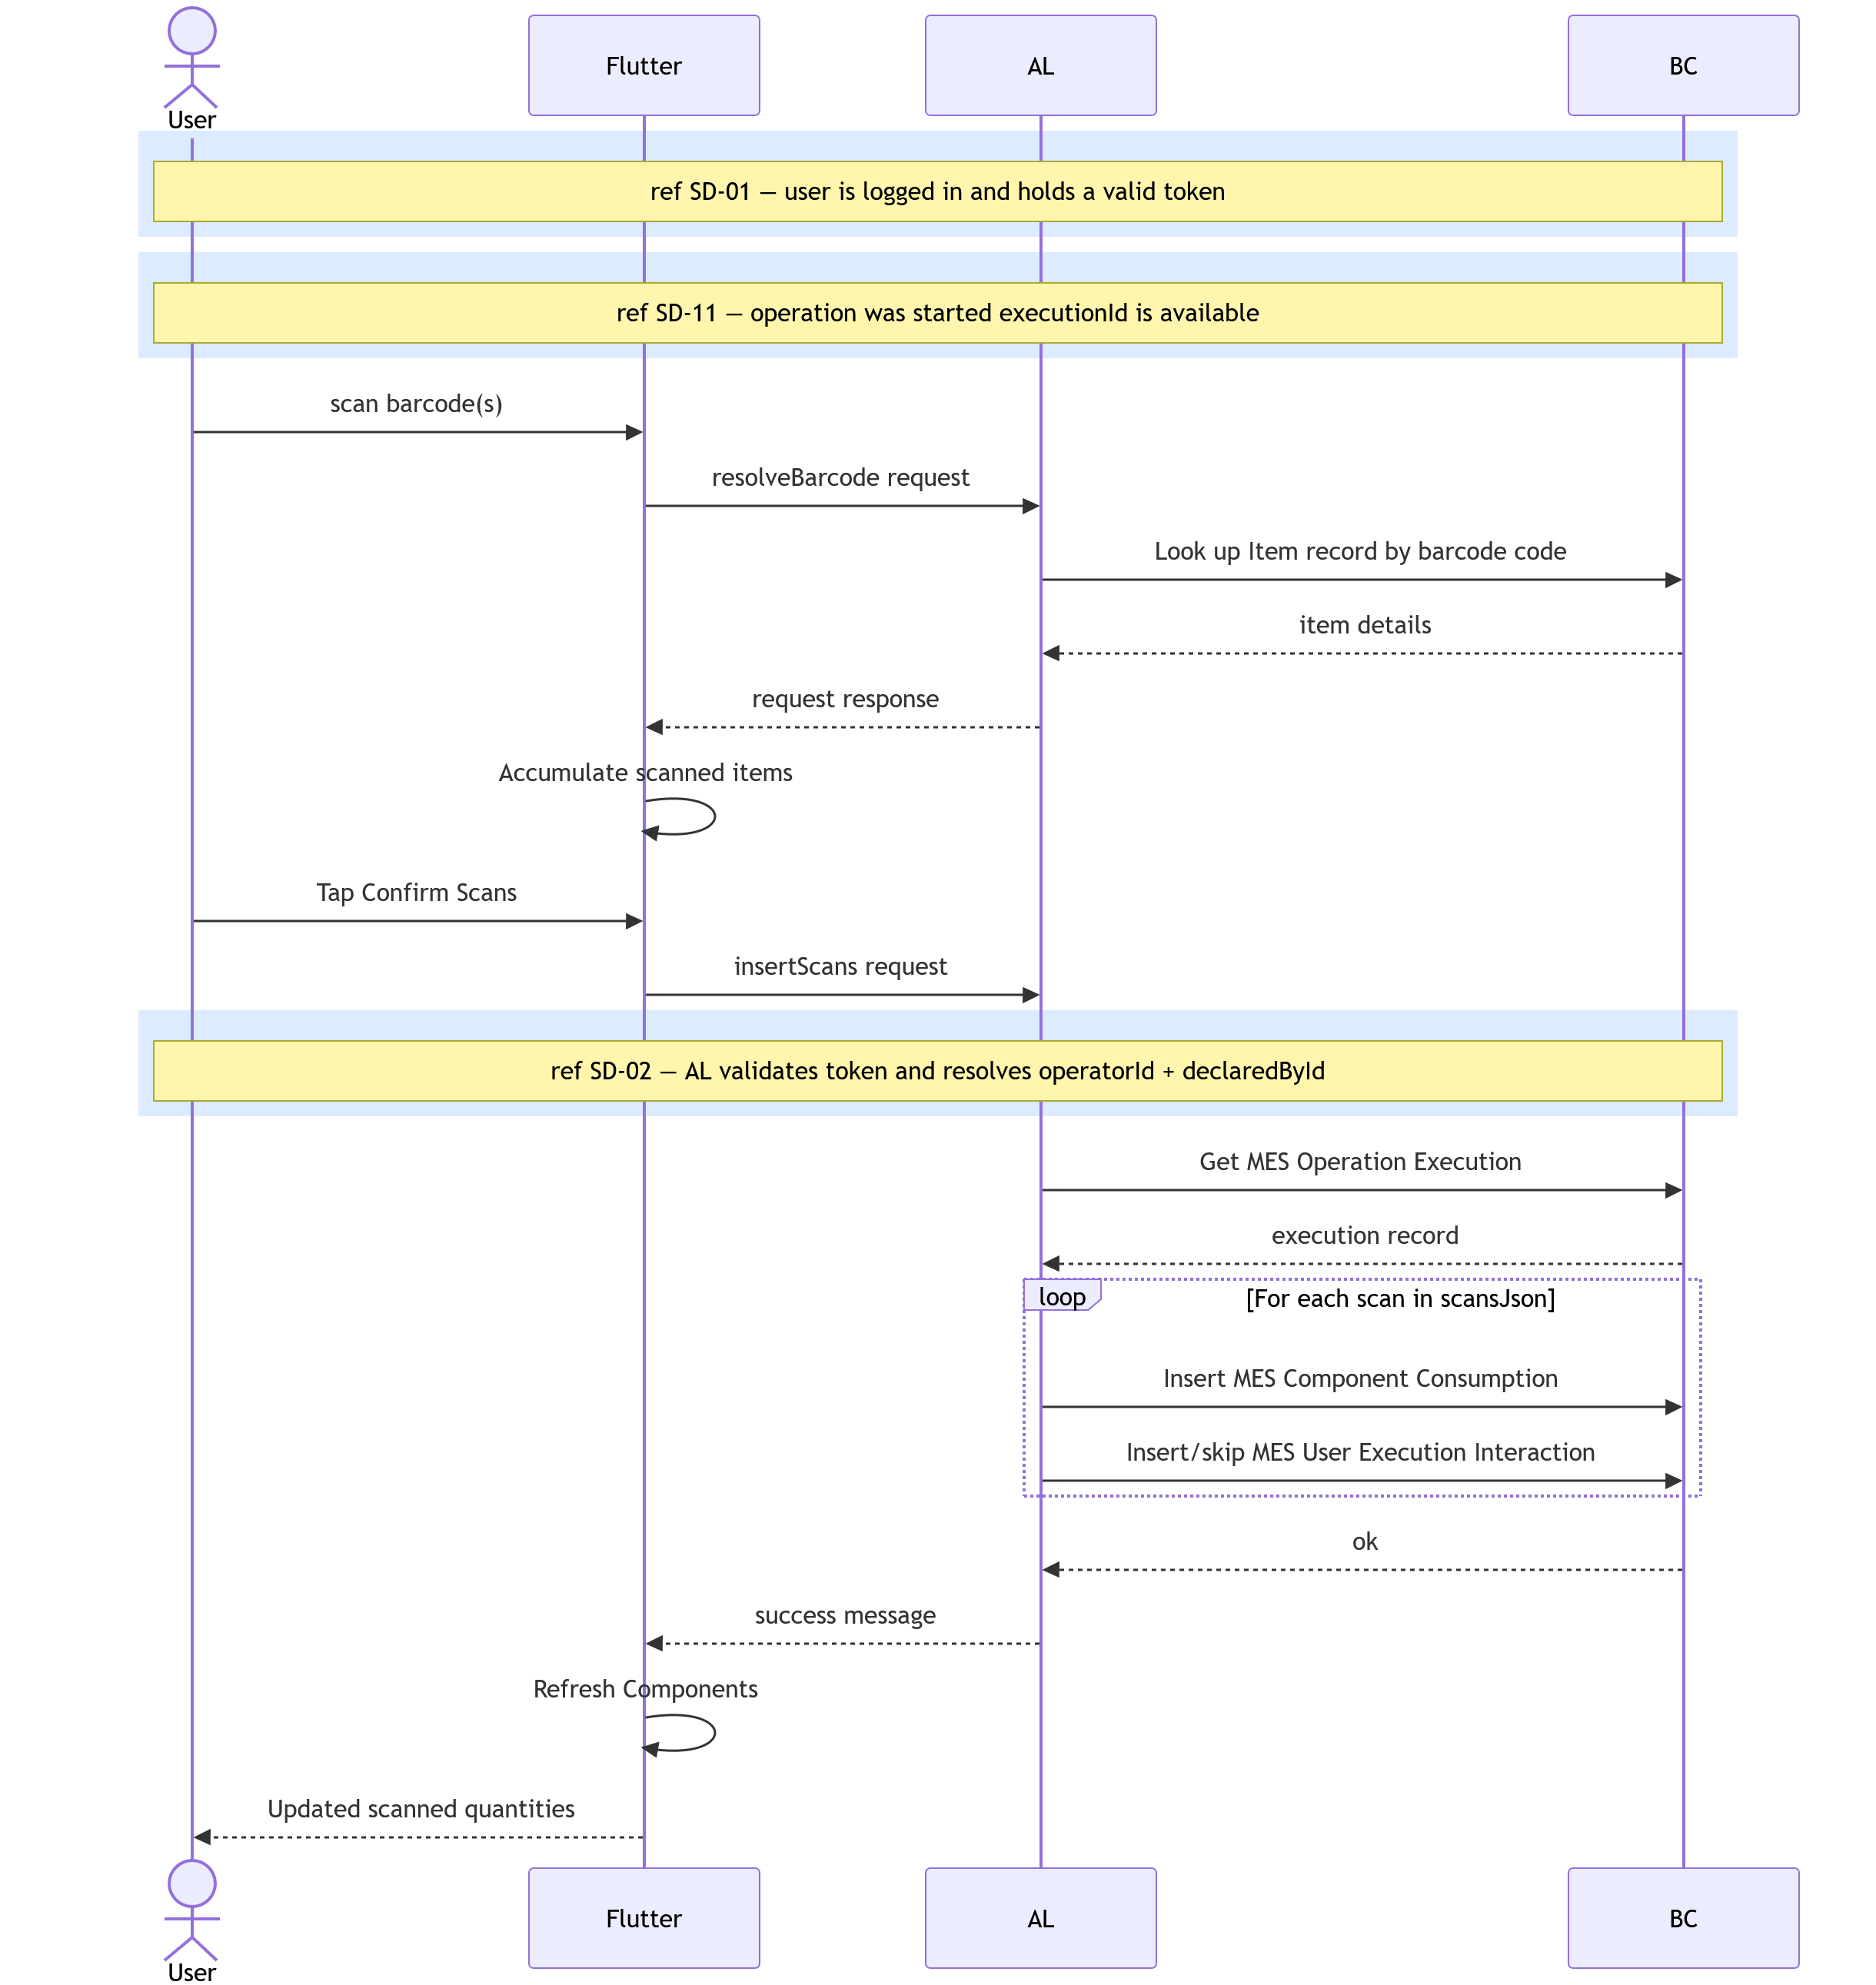
\includegraphics[width=\linewidth,height=0.82\textheight,keepaspectratio]{./media/MES_Sprint-3-Repport/diagrams/sequence/scan-component.png}
%   \caption{SD-17: scan component.}
%   \label{fig:s3-seq-scan-component}
% \end{figure}

%=====SD-17==========================================================
% sequenceDiagram
%       actor User
%       participant Flutter
%       participant Node as Node.js Middleware
%       participant AL
%       participant BC

%       rect rgb(220,235,255)
%           Note over User,BC: ref SD-01 — user is logged in and holds a valid token
%       end
%       rect rgb(220,235,255)
%           Note over User,BC: ref SD-11 — operation was started, executionId available
%       end

%       User->>Flutter: Tap Scan Item and Scan barcode with camera
%       Flutter->>Node: POST /api/resolveBarcode
%       Node->>AL: MESWebService_resolveBarcode

%       alt Barcode contains 'Item Number:' prefix 
%           AL->>AL: Parse Item No. from barcode string
%           AL->>BC: get the item record
%           BC-->>AL: item record 
%           AL->>BC: resolve canonical identifier
%       else Standard barcode
%           AL->>BC: resolve the identifier from Item Identifier
%       end
%       AL->>BC: get the item record
%       AL->>BC: Item Unit of Measure.Get(itemNo, unitOfMeasureCode) → quantityPerUnitOfMeasure
%       BC-->>AL: itemNo, itemDescription, unitOfMeasure, quantityPerUnitOfMeasure
%       AL-->>Node: response
%       Node-->>Flutter: response

%       Flutter->>Flutter: validation
%       Flutter->>Flutter: Add or increment item in local scanned items list
%       Flutter-->>User: Item shown in scan list

%       User->>Flutter: Tap Confirm Scans
%       Flutter->>Node: POST /api/insertScans 
%       Node->>AL: MESWebService_insertScans 

%       rect rgb(220,235,255)
%           Note over AL,BC: ref SD-02 — ValidateToken called
%       end

%       AL->>BC: get the execution record of the operation
%       BC-->>AL: execution record

%       loop For each scan in scansJson
%           AL->>BC: Insert MES Component Consumption 
%           AL->>BC: get the item record
%           AL->>BC: Insert Item Journal Line
%       end

%       AL->>BC: post all journal lines to BC inventory
%       BC-->>AL: ok
%       AL-->>Node: success response
%       Node-->>Flutter: success response
%       Flutter->>Flutter: trigger refresh and pops ScannerWidget
%       Flutter-->>User: Updated Required Component widget
%====================================================================

Figure~\ref{fig:s3-seq-fetch-operation-live-data} presents the live operation
data retrieval sequence. When the user navigates to the
\uilabel{OperationDetailPage}, three \techname{StreamBuilder} instances mount
simultaneously: one polling the current operation status and quantities from
\techname{Business Central} (SD-18), one consuming the production-cycle stream
(SD-22), and one consuming the BOM stream (SD-21). The \techname{Flutter}
client merges all three data sources and renders the full detail view. If the
operation is finished, cancelled, or not yet started, the live-data stream
returns an empty response and the client falls back to the history view.

\begin{figure}[H]
  \centering
  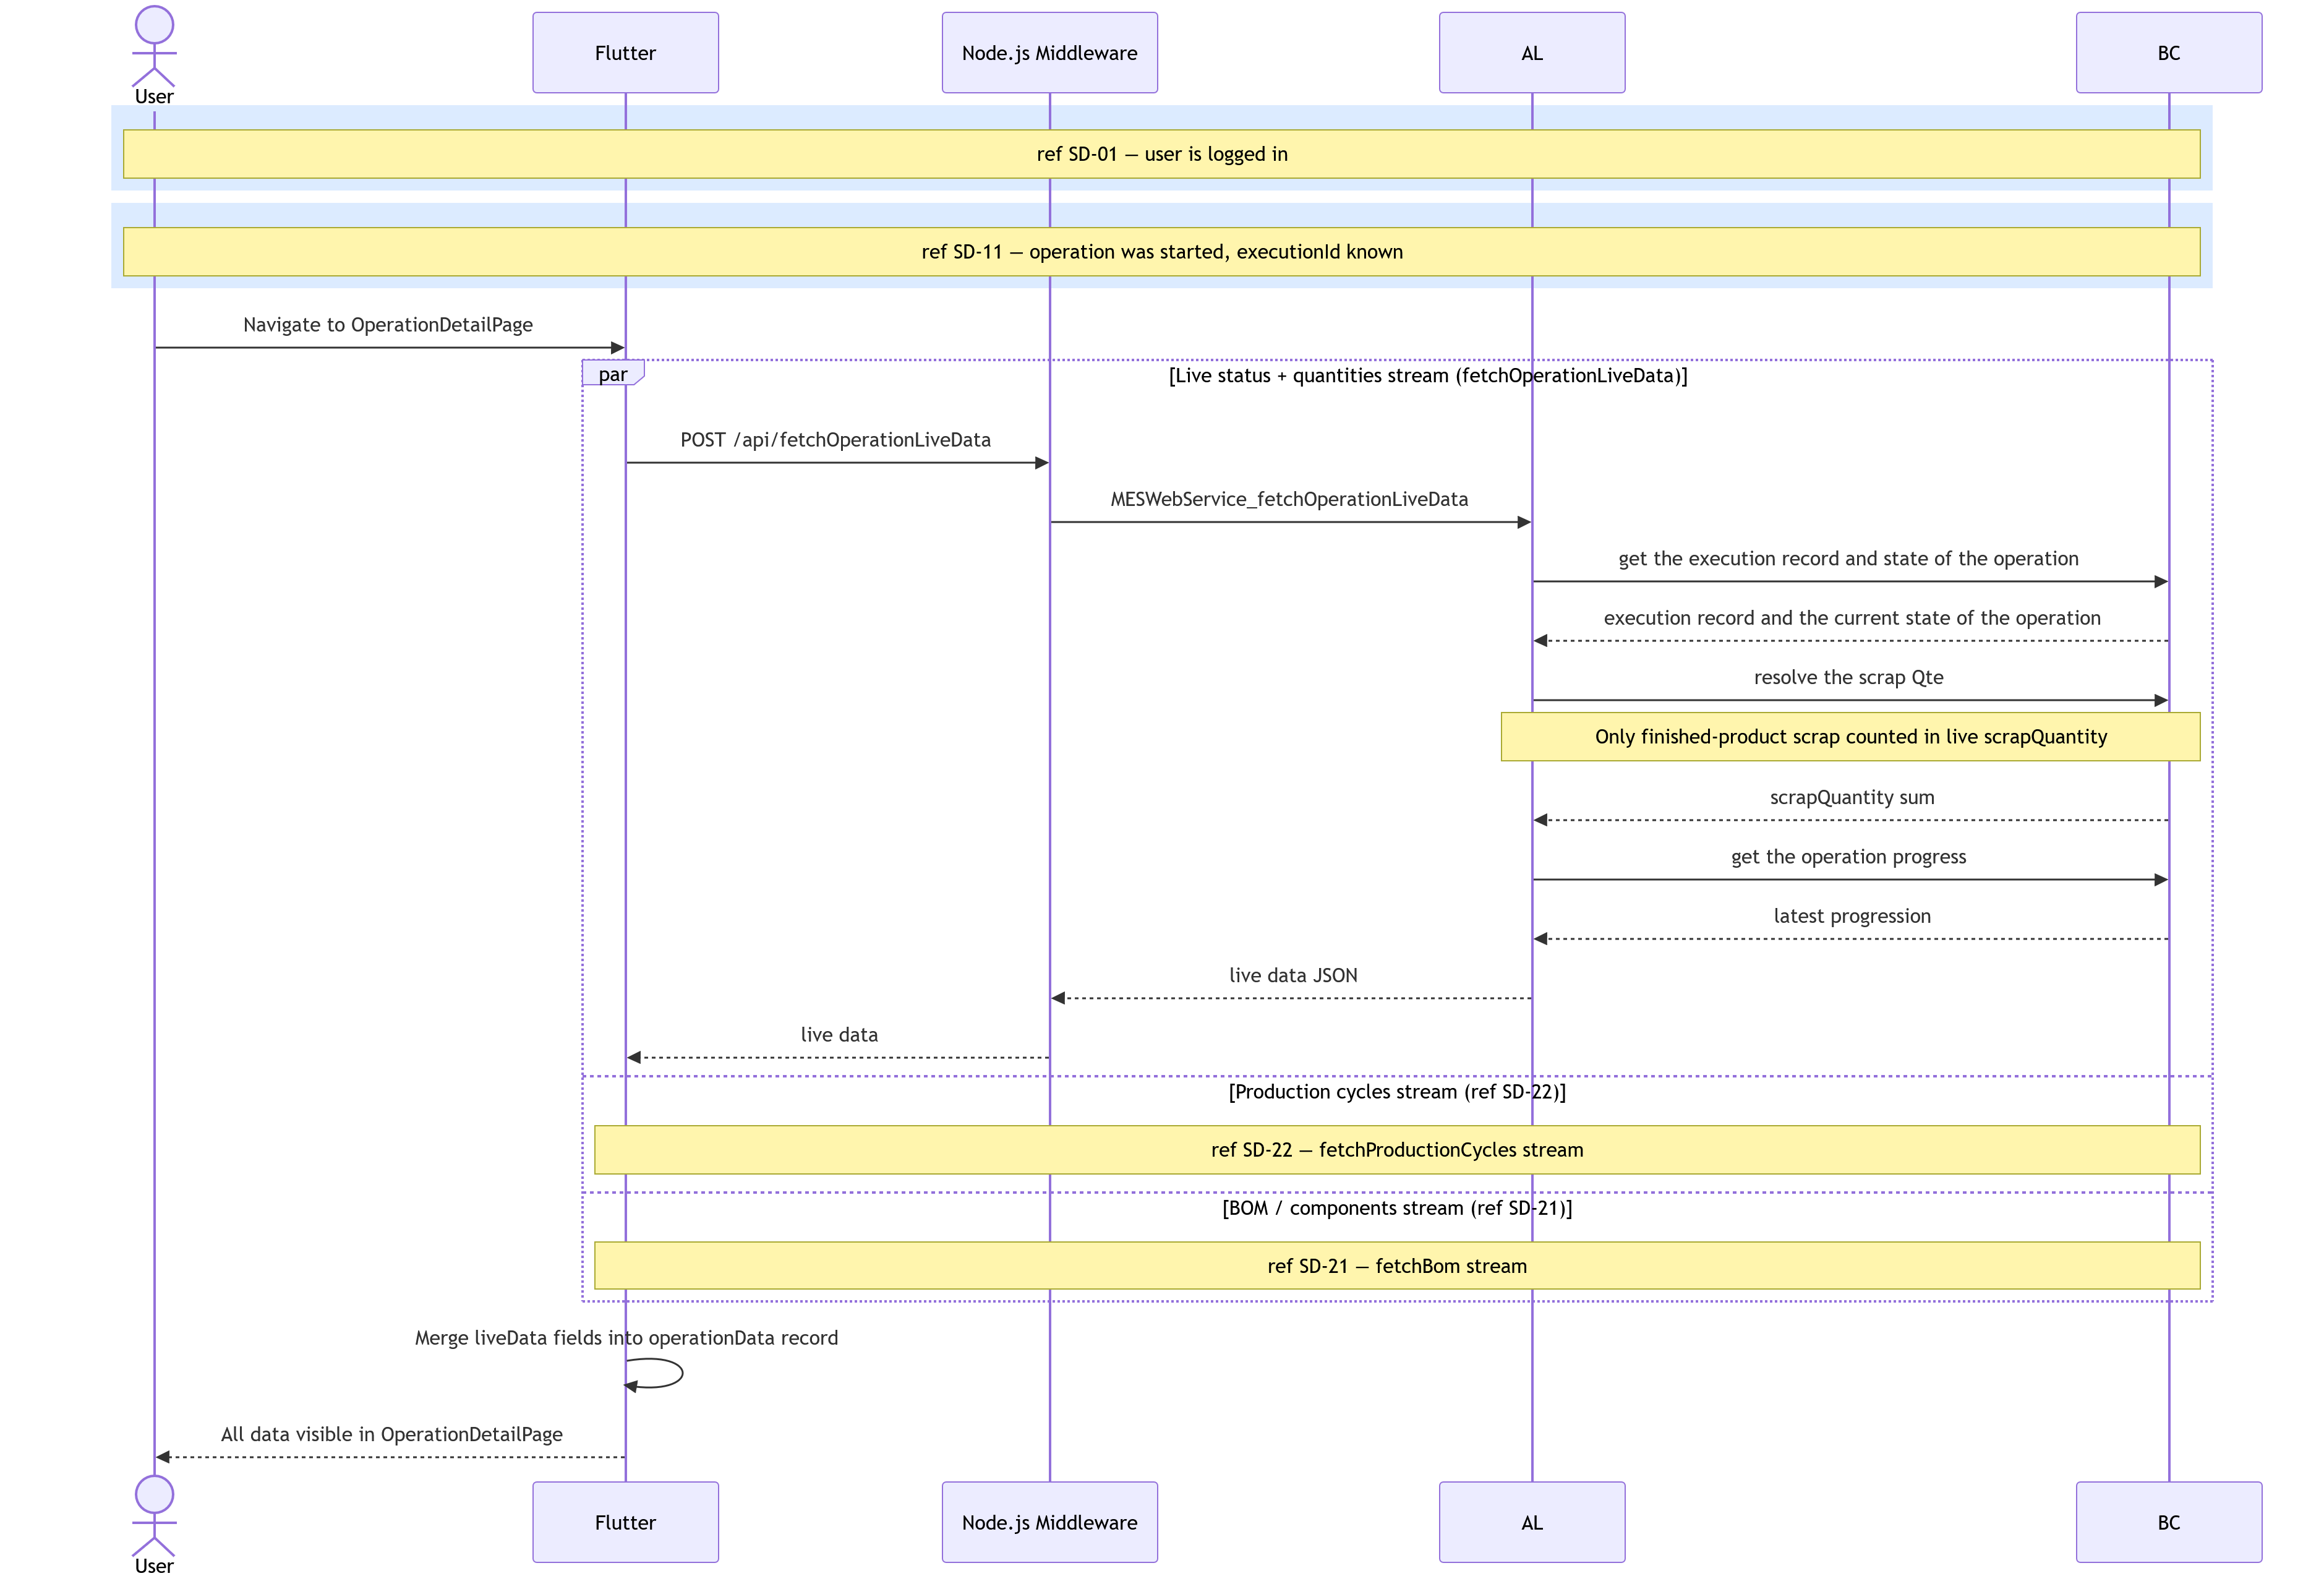
\includegraphics[width=\linewidth,height=0.82\textheight,keepaspectratio]{./media/MES_Sprint-3-Repport/diagrams/sequence/fetch-operation-live-data.png}
  \caption{SD-18: Fetch Operation Live Data.}
  \label{fig:s3-seq-fetch-operation-live-data}
\end{figure}

%=====SD-18==========================================================
%  sequenceDiagram
%       actor User
%       participant Flutter
%       participant Node as Node.js Middleware
%       participant AL
%       participant BC

%       rect rgb(220,235,255)
%           Note over User,BC: ref SD-01 — user is logged in
%       end
%       rect rgb(220,235,255)
%           Note over User,BC: ref SD-11 — operation was started, executionId known
%       end

%       User->>Flutter: Navigate to OperationDetailPage

%       par Live status + quantities stream (fetchOperationLiveData)
%           Flutter->>Node: POST /api/fetchOperationLiveData 
%           Node->>AL: MESWebService_fetchOperationLiveData 
%           AL->>BC: get the execution record and state of the operation
%           BC-->>AL: execution record and the current state of the operation
%           AL->>BC: resolve the scrap Qte
%           Note over AL,BC: Only finished-product scrap counted in live scrapQuantity
%           BC-->>AL: scrapQuantity sum
%           AL->>BC:get the operation progress
%           BC-->>AL: latest progression
%           AL-->>Node: live data JSON
%           Node-->>Flutter: live data
%       and Production cycles stream (ref SD-22)
%           Note over Flutter,BC: ref SD-22 — fetchProductionCycles stream
%       and BOM / components stream (ref SD-21)
%           Note over Flutter,BC: ref SD-21 — fetchBom stream
%       end

%       Flutter->>Flutter: Merge liveData fields into operationData record
%       Flutter-->>User: All data visible in OperationDetailPage
%====================================================================


\subsection{Class Diagram}

The UML Class Diagram (Figure~\ref{fig:s3-class-diagram-s3}) extends the Sprint~2
domain model with three new tables. \modulename{MES Operation Execution} (50110)
is the central anchor record linking a machine, production order, and operation
to its full lifecycle; it holds item description, order quantity, and start/end
timestamps. \modulename{MES Operation Progression} (50109) is an append-only
table of production cycle declarations, each referencing an execution and
accumulating \texttt{TotalProducedQuantity} from the previous cycle.
\modulename{MES Component Consumption} (50111) records scrap and barcode scan
events, also referencing an execution. Both progression and consumption records
are child tables of the execution record, forming a hub-and-spoke traceability
model.

\begin{figure}[H]
  \centering
  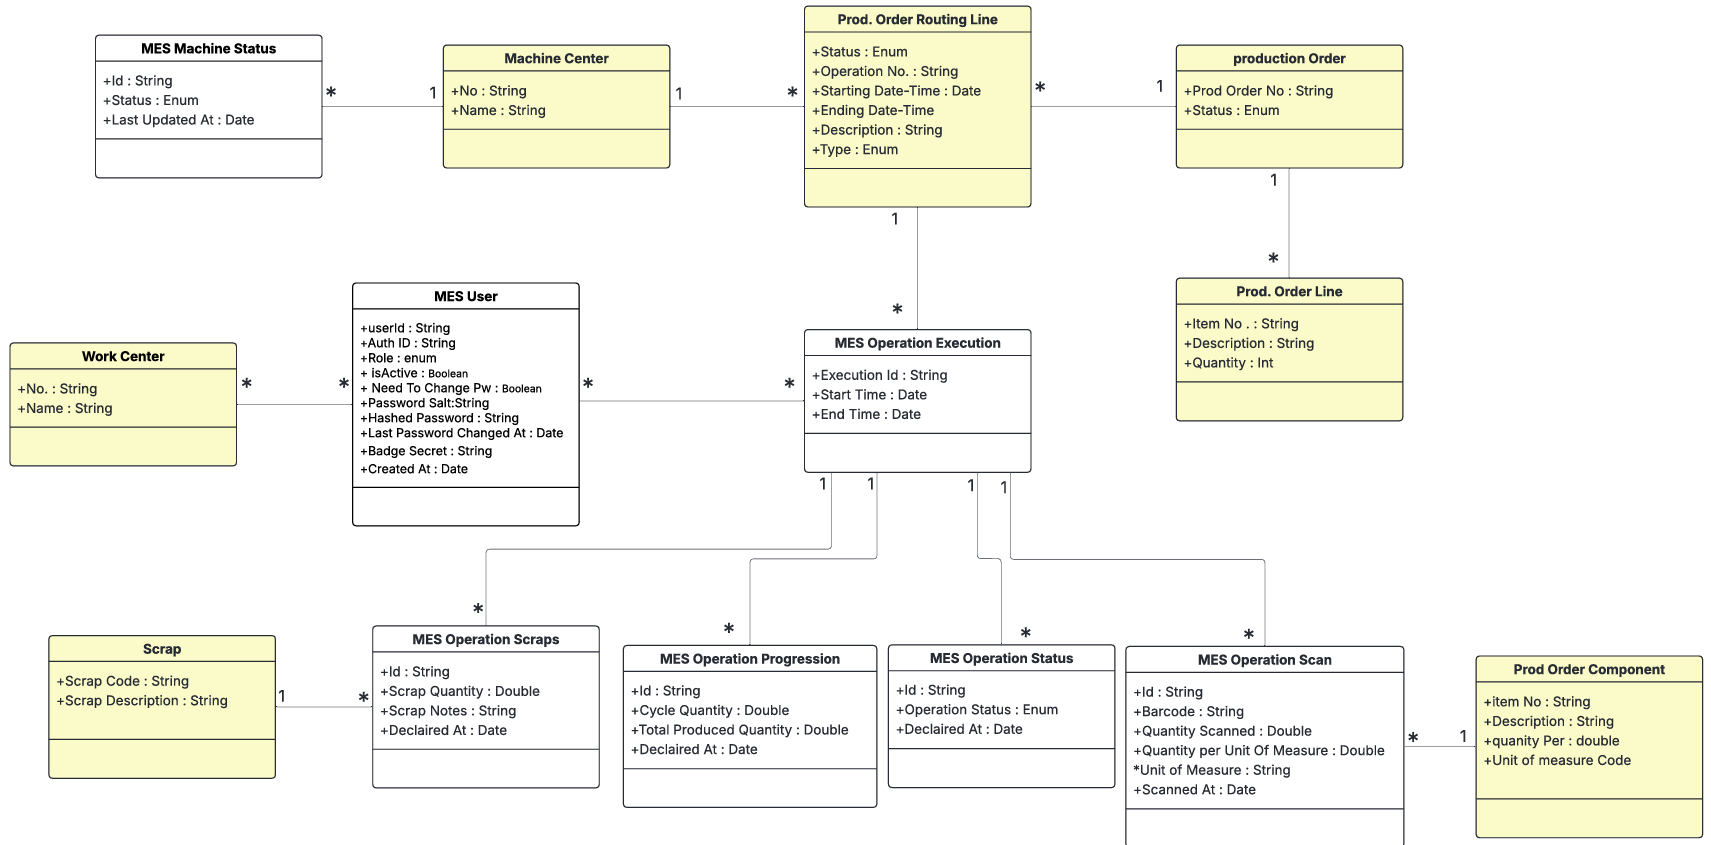
\includegraphics[width=\linewidth,keepaspectratio]{./media/MES_Sprint-3-Repport/diagrams/class/sprint3.png}
  \caption{UML Class Diagram --- Production Execution \& Traceability.}
  \label{fig:s3-class-diagram-s3}
\end{figure}

% ---------------------------------------------------------------------------
% 4. IMPLEMENTATION
% ---------------------------------------------------------------------------
\section{Implementation}

\subsection{Backend Implementation}
\subsubsection{Tables and Entities}

\begin{longtable}{@{} P{0.21\linewidth} P{0.17\linewidth} P{0.57\linewidth} @{}}
	\caption{MES Operation Execution (Table 50110) --- Field Dictionary}
	\label{tab:s3-table-execution} \\
	\toprule
	\textbf{Name} & \textbf{Type} & \textbf{Description} \\
	\midrule
	\endfirsthead
	\toprule
	\textbf{Name} & \textbf{Type} & \textbf{Description} \\
	\midrule
	\endhead
	
	\multicolumn{3}{r}{\small Continued on next page} \\
	\endfoot
	\bottomrule
	\endlastfoot
	
	Execution Id & Code[50] & GUID-based primary key; auto-generated on insert. \\
	\midrule
	Machine No & Code[20] & References Machine Center (no referential constraint enforced in the current implementation). \\
	\midrule
	Prod Order No & Code[20] & Foreign key to Prod.\ Order Routing Line. \\
	\midrule
	Operation No & Code[10] & Operation identifier from the routing line. \\
	\midrule
	Item No & Code[20] & Copied from Prod.\ Order Line on execution creation. \\
	\midrule
	Item Description & Text[100] & Copied from Prod.\ Order Line for denormalized display. \\
	\midrule
	Order Quantity & Decimal & Copied from Prod.\ Order Line; used for progress calculation. \\
	\midrule
	Start Time & DateTime & Set by \texttt{OnInsert} trigger to \texttt{CurrentDateTime()}. \\
	\midrule
	End Time & DateTime & Stamped when status transitions to Finished or Cancelled. \\
\end{longtable}

\begin{longtable}{@{} P{0.21\linewidth} P{0.17\linewidth} P{0.57\linewidth} @{}}
	\caption{MES Operation Progression (Table 50109) --- Field Dictionary}
	\label{tab:s3-table-progression} \\
	\toprule
	\textbf{Name} & \textbf{Type} & \textbf{Description} \\
	\midrule
	\endfirsthead
	\toprule
	\textbf{Name} & \textbf{Type} & \textbf{Description} \\
	\midrule
	\endhead
	\multicolumn{3}{r}{\small Continued on next page} \\
	\endfoot
	\bottomrule
	\endlastfoot
	
	Id & Code[50] & GUID-based primary key; auto-generated on insert. \\
	\midrule
	Execution Id & Code[50] & Foreign key to MES Operation Execution. \\
	\midrule
	Cycle Quantity & Decimal & Units declared in this single production cycle. \\
	\midrule
	Total Produced Quantity & Decimal & Running total: previous total + Cycle Quantity. \\
	\midrule
	Operator Id & Code[50] & BC session UserId of the user who produced the unites during this cycle. \\
	\midrule
	Declared At & DateTime & Set by \texttt{OnInsert} trigger to \texttt{CurrentDateTime()}. \\
	\midrule
	Declared By & Code[50] &  BC session UserId of the user who declared the production cycle  \\
\end{longtable}

\begin{longtable}{@{} P{0.21\linewidth} P{0.17\linewidth} P{0.57\linewidth} @{}}
	\caption{MES Operation Scan (Table 50111) --- Field Dictionary}
	\label{tab:s3-table-consumption} \\
	\toprule
	\textbf{Name} & \textbf{Type} & \textbf{Description} \\
	\midrule
	\endfirsthead
	\toprule
	\textbf{Name} & \textbf{Type} & \textbf{Description} \\
	\midrule
	\endhead
	\multicolumn{3}{r}{\small Continued on next page} \\
	\endfoot
	\endlastfoot
	
	Id & Code[50] & GUID-based primary key; auto-generated on insert. \\
	\midrule
	Execution Id & Code[50] & Foreign key to MES Operation Execution. \\
	\midrule
	Prod Order No & Code[50] & Foreign key to Prod.\ Order Component. \\
	\midrule
	Item No & Code[50] & Item identifier of the consumed component. \\
	\midrule
	Barcode & Text[500] & Barcode scanned to register the component. \\
	\midrule
	Unit of Measure & Code[50] & Unit of measure code from the component definition. \\
	\midrule
	Quantity Scanned & Decimal & Raw quantity read from the barcode scan. \\
	\midrule
	Quantity per Unit of Measure & Decimal & Unit-of-measure conversion factor; the effective consumed quantity equals Quantity Scanned multiplied by this value. \\	
	\midrule
	Operator Id & Code[50] & BC session UserId of the operator who scanned. \\
	\midrule
	Scanned At & DateTime & Set by \texttt{OnInsert} trigger to \texttt{CurrentDateTime()}. \\
	\midrule
	Declared By & Code[50] &  BC session UserId of the user who declared the production cycle  \\
	\midrule
\end{longtable}


\subsubsection{REST API and Web Services Implementation}

All endpoints are exposed as ODataV4 unbound actions through
\techname{MES Web Service} (codeunit~50126) and are served by the
middleware at:

\begin{center}
  \texttt{middlewareHostURL/api/<endpointName>}
\end{center}

\noindent Each request is forwarded to the \techname{AL} layer as an
ODataV4 action call of the form:

\begin{center}
  \texttt{POST~<baseUrl>/ODataV4/MESWebService\_<ProcedureName>?company=<companyId>}
\end{center}

\noindent Table~\ref{tab:s3-api-endpoints} lists all endpoints introduced
in this sprint.

\begin{longtable}{@{} P{0.48\linewidth} @{\hspace{0.04\linewidth}} P{0.48\linewidth} @{}}
  \caption{New API Endpoints --- Sprint 3}
  \label{tab:s3-api-endpoints}\\
  \toprule
  \textbf{Endpoint} & \textbf{Endpoint}\\
  \midrule
  \endfirsthead
  \toprule
  \textbf{Endpoint} & \textbf{Endpoint}\\
  \midrule
  \endhead
  \multicolumn{2}{r}{\small Continued on next page}\\
  \endfoot
  \bottomrule
  \endlastfoot

  \apiendpoint{startOperation}         & \apiendpoint{fetchOperationsStatusAndProgress} \\
  \midrule
  \apiendpoint{declareProduction}      & \apiendpoint{fetchOperationLiveData}            \\
  \midrule
  \apiendpoint{pauseOperation}         & \apiendpoint{fetchProductionCycles}             \\
  \midrule
  \apiendpoint{resumeOperation}        & \apiendpoint{fetchBom}                          \\
  \midrule
  \apiendpoint{finishOperation}        &                                                  \\
  \midrule
  \apiendpoint{cancelOperation}        &                                                  \\
\end{longtable}
\subsection{Frontend Implementation}

This sprint introduces a reactive pattern: a shared \texttt{StreamController<void>.broadcast()}
in \techname{MachineOrdersProvider} and \techname{MesComponentConsumptionProvider}. When any write
action (declare, pause, resume, finish, cancel) succeeds, \texttt{triggerRefresh()} adds an event 
to the controller. All live data streams (\texttt{fetchOperationLiveDataStream}, 
\texttt{streamProductionCycles}, \texttt{streamBom}) are implemented as \texttt{async*} generators
that yield on both the initial fetch and on each event from the shared broadcast stream, enabling 
coordinated, push-driven UI updates without polling.

\subsubsection{Provider Architecture}

\begin{longtable}{@{} P{0.30\linewidth} P{0.65\linewidth} @{}}
	\caption{Provider Responsibilities --- Sprint 3 Additions}
	\label{tab:s3-providers}\\
	\toprule
	\textbf{Provider}& \textbf{Responsibility}\\
	\midrule
	\endfirsthead
	\toprule
	\textbf{Provider}& \textbf{Responsibility}\\
	\midrule
	\endhead
	\multicolumn{2}{r}{\small Continued on next page}\\
	\endfoot
	\bottomrule
	\endlastfoot
	
	\techname{MachineOrdersProvider} & Owns write operations (start, declare, pause, resume, finish, cancel) and their refresh controller; exposes all live data streams. \\
	\midrule
	\techname{MesComponentConsumption\allowbreak Provider} & Exposes \texttt{getBomStream()} combining service fetch with an independent refresh controller.\\
	\midrule
	\techname{AuthProvider}& Adds \texttt{changePassword()} and \texttt{adminSetPassword()}; manages \texttt{needsPasswordChange} flag in the in-memory session. \\
\end{longtable}

\subsubsection{User Interface}
Figures~\ref{fig:s3-ui-op-detail-running} through~\ref{fig:s3-ui-op-detail-cancelled} illustrate the \uilabel{Operation Detail Page}
across its five possible states: Running, Paused, Finished, Interrupted, and Cancelled. Each view adapts its action buttons and status badge
to the current state, while the production chart, cycle table, and BOM list remain consistently visible. On desktop, the page 
uses a two-column layout with order information and production data on the left, and the \uilabel{Quick Actions} panel on the
right; on mobile, these sections stack vertically. Action button availability is state-dependent: \uilabel{Declare Production} 
and \uilabel{Declare Scrap} are disabled in the Paused, Finished, and Cancelled states; the close button triggers a 
\uilabel{Finish Production Order} or \uilabel{Interrupt Production Order} action depending on whether the progress has reached 100\%;
and \uilabel{Print Label} is enabled only once the operation is finished.

\begin{figure}[H]
    \centering
    \setlength{\fboxsep}{5pt}
    \colorbox{black}{%
        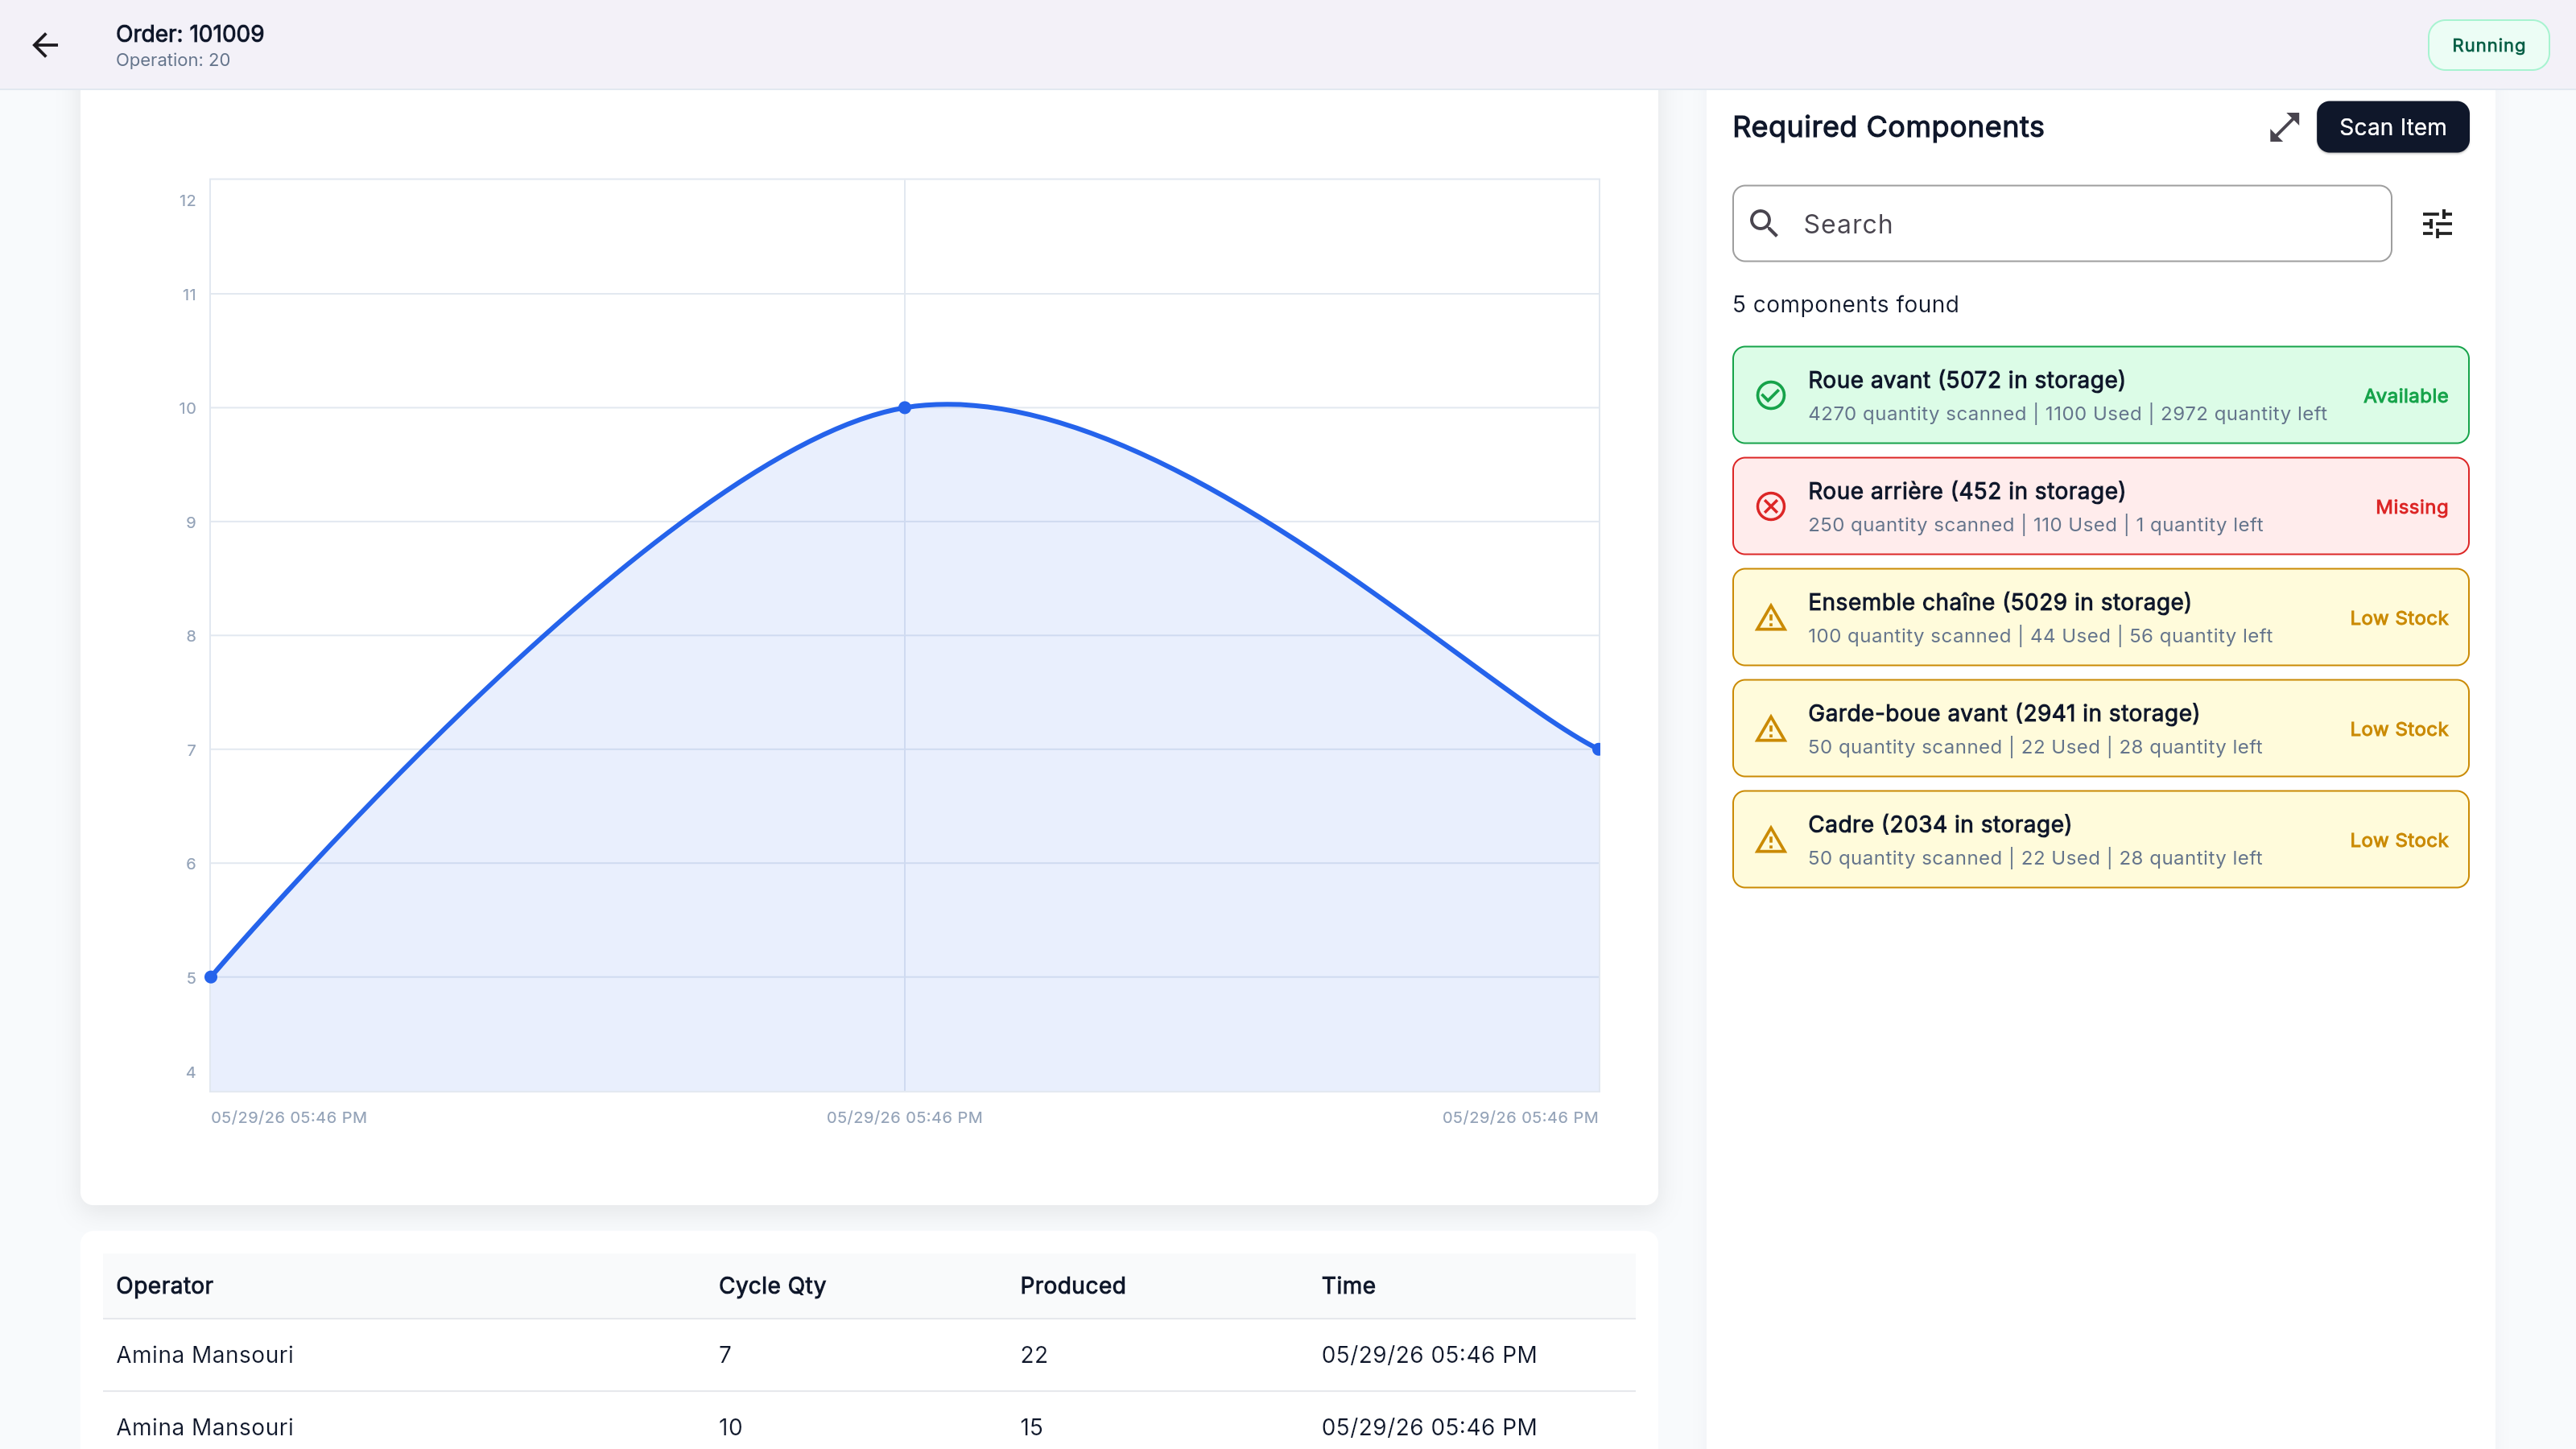
\includegraphics[height=0.3\textheight,keepaspectratio]{./media/MES_Sprint-3-Repport/UI/opDetailRunning/wide.png}%
        \hspace{\fboxsep}%
        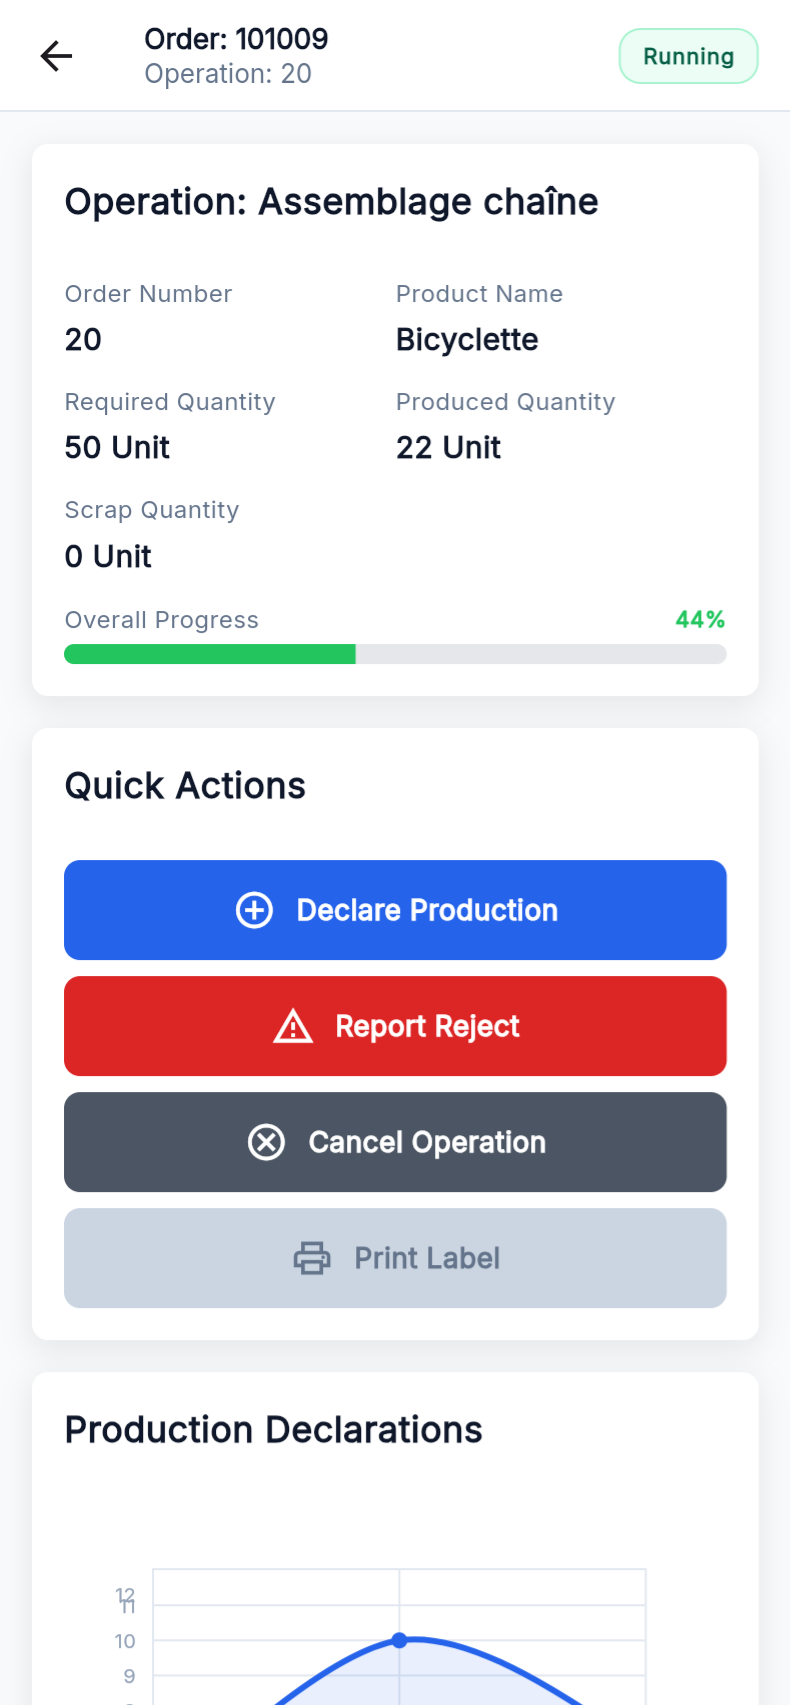
\includegraphics[height=0.3\textheight,keepaspectratio]{./media/MES_Sprint-3-Repport/UI/opDetailRunning/small.png}%
    }
    \caption{\uilabel{Operation Detail Page} (Running state) --- desktop and mobile views.}
    \label{fig:s3-ui-op-detail-running}
\end{figure}


\begin{figure}[H]
	\centering
	\setlength{\fboxsep}{5pt}
	\colorbox{black}{%
		
\includegraphics[height=0.3\textheight,keepaspectratio]{./media/MES_Sprint-3-Repport/placeholder-image.png}%
		\hspace{\fboxsep}%
		
\includegraphics[height=0.3\textheight,keepaspectratio]{./media/MES_Sprint-3-Repport/placeholder-image.png}%
	}
	\caption{\uilabel{Operation Detail Page} (Cancelled state) --- desktop and mobile views.}
	\label{fig:s3-ui-op-detail-cancelled}
\end{figure}

\section{Test and Validation}
\subsection{Integration test}

For integration testing, we chose Postman, a powerful and user-friendly tool for API evaluation. Figure~\ref{fig:s3-test-postman-fetchBom} shows a test case for the \apiendpoint{/fetchBom} endpoint.

\begin{figure}[H]
  \centering
  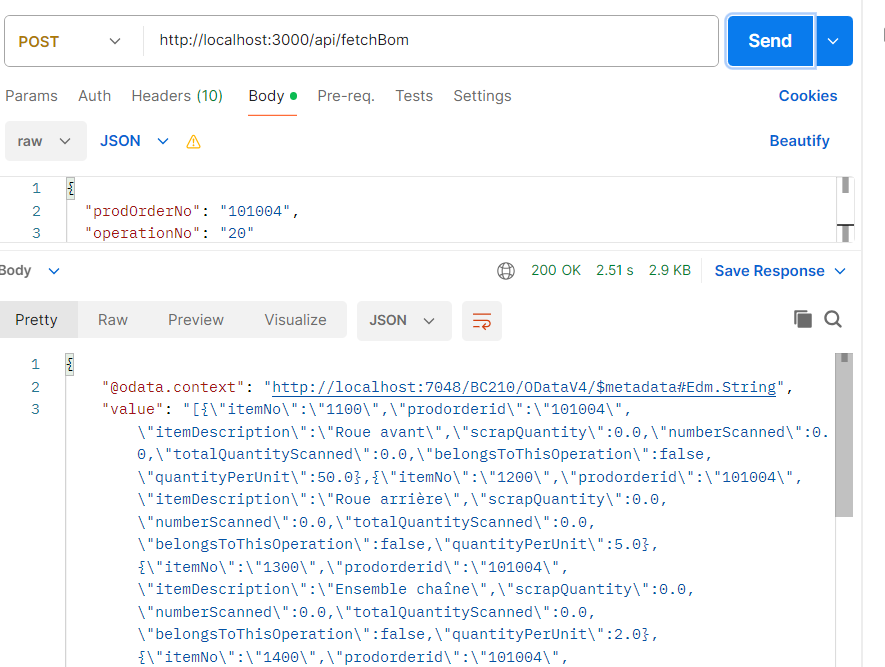
\includegraphics[width=\linewidth,keepaspectratio]{./media/MES_Sprint-3-Repport/test/postman/fetchBom.png}
  \caption{Postman endpoint test --- fetchBom.}
  \label{fig:s3-test-postman-fetchBom}
\end{figure}

\phantomsection
\section*{Conclusion}
\addcontentsline{toc}{section}{Conclusion}

This sprint delivered the complete shop-floor execution loop for the MES system.
Operators can now start, pause, resume, interrupt and close production operations, declare
production output cycle by cycle, track cumulative progress through real-time
charts and paginated tables, inspect the Bill of Materials, scan physical components
via barcodes, declare scrapped units with reason codes, and print
traceable labels for both production orders and individual declared units.
Supervisors gain the ability to declare production on behalf of a specific operator,
with a full attribution audit trail. The reactive stream architecture ensures that
all UI panels update in concert after every write action, providing a consistent
and accurate view of the production floor without manual refreshes.
